\documentclass[1p]{elsarticle_modified}
%\bibliographystyle{elsarticle-num}

%\usepackage[colorlinks]{hyperref}
%\usepackage{abbrmath_seonhwa} %\Abb, \Ascr, \Acal ,\Abf, \Afrak
\usepackage{amsfonts}
\usepackage{amssymb}
\usepackage{amsmath}
\usepackage{amsthm}
\usepackage{scalefnt}
\usepackage{amsbsy}
\usepackage{kotex}
\usepackage{caption}
\usepackage{subfig}
\usepackage{color}
\usepackage{graphicx}
\usepackage{xcolor} %% white, black, red, green, blue, cyan, magenta, yellow
\usepackage{float}
\usepackage{setspace}
\usepackage{hyperref}

\usepackage{tikz}
\usetikzlibrary{arrows}

\usepackage{multirow}
\usepackage{array} % fixed length table
\usepackage{hhline}

%%%%%%%%%%%%%%%%%%%%%
\makeatletter
\renewcommand*\env@matrix[1][\arraystretch]{%
	\edef\arraystretch{#1}%
	\hskip -\arraycolsep
	\let\@ifnextchar\new@ifnextchar
	\array{*\c@MaxMatrixCols c}}
\makeatother %https://tex.stackexchange.com/questions/14071/how-can-i-increase-the-line-spacing-in-a-matrix
%%%%%%%%%%%%%%%

\usepackage[normalem]{ulem}

\newcommand{\msout}[1]{\ifmmode\text{\sout{\ensuremath{#1}}}\else\sout{#1}\fi}
%SOURCE: \msout is \stkout macro in https://tex.stackexchange.com/questions/20609/strikeout-in-math-mode

\newcommand{\cancel}[1]{
	\ifmmode
	{\color{red}\msout{#1}}
	\else
	{\color{red}\sout{#1}}
	\fi
}

\newcommand{\add}[1]{
	{\color{blue}\uwave{#1}}
}

\newcommand{\replace}[2]{
	\ifmmode
	{\color{red}\msout{#1}}{\color{blue}\uwave{#2}}
	\else
	{\color{red}\sout{#1}}{\color{blue}\uwave{#2}}
	\fi
}

\newcommand{\Sol}{\mathcal{S}} %segment
\newcommand{\D}{D} %diagram
\newcommand{\A}{\mathcal{A}} %arc


%%%%%%%%%%%%%%%%%%%%%%%%%%%%%5 test

\def\sl{\operatorname{\textup{SL}}(2,\Cbb)}
\def\psl{\operatorname{\textup{PSL}}(2,\Cbb)}
\def\quan{\mkern 1mu \triangleright \mkern 1mu}

\theoremstyle{definition}
\newtheorem{thm}{Theorem}[section]
\newtheorem{prop}[thm]{Proposition}
\newtheorem{lem}[thm]{Lemma}
\newtheorem{ques}[thm]{Question}
\newtheorem{cor}[thm]{Corollary}
\newtheorem{defn}[thm]{Definition}
\newtheorem{exam}[thm]{Example}
\newtheorem{rmk}[thm]{Remark}
\newtheorem{alg}[thm]{Algorithm}

\newcommand{\I}{\sqrt{-1}}
\begin{document}

%\begin{frontmatter}
%
%\title{Boundary parabolic representations of knots up to 8 crossings}
%
%%% Group authors per affiliation:
%\author{Yunhi Cho} 
%\address{Department of Mathematics, University of Seoul, Seoul, Korea}
%\ead{yhcho@uos.ac.kr}
%
%
%\author{Seonhwa Kim} %\fnref{s_kim}}
%\address{Center for Geometry and Physics, Institute for Basic Science, Pohang, 37673, Korea}
%\ead{ryeona17@ibs.re.kr}
%
%\author{Hyuk Kim}
%\address{Department of Mathematical Sciences, Seoul National University, Seoul 08826, Korea}
%\ead{hyukkim@snu.ac.kr}
%
%\author{Seokbeom Yoon}
%\address{Department of Mathematical Sciences, Seoul National University, Seoul, 08826,  Korea}
%\ead{sbyoon15@snu.ac.kr}
%
%\begin{abstract}
%We find all boundary parabolic representation of knots up to 8 crossings.
%
%\end{abstract}
%\begin{keyword}
%    \MSC[2010] 57M25 
%\end{keyword}
%
%\end{frontmatter}

%\linenumbers
%\tableofcontents
%
\newcommand\colored[1]{\textcolor{white}{\rule[-0.35ex]{0.8em}{1.4ex}}\kern-0.8em\color{red} #1}%
%\newcommand\colored[1]{\textcolor{white}{ #1}\kern-2.17ex	\textcolor{white}{ #1}\kern-1.81ex	\textcolor{white}{ #1}\kern-2.15ex\color{red}#1	}

{\Large $\underline{12a_{0588}~(K12a_{0588})}$}

\setlength{\tabcolsep}{10pt}
\renewcommand{\arraystretch}{1.6}
\vspace{1cm}\begin{tabular}{m{100pt}>{\centering\arraybackslash}m{274pt}}
\multirow{5}{120pt}{
	\centering
	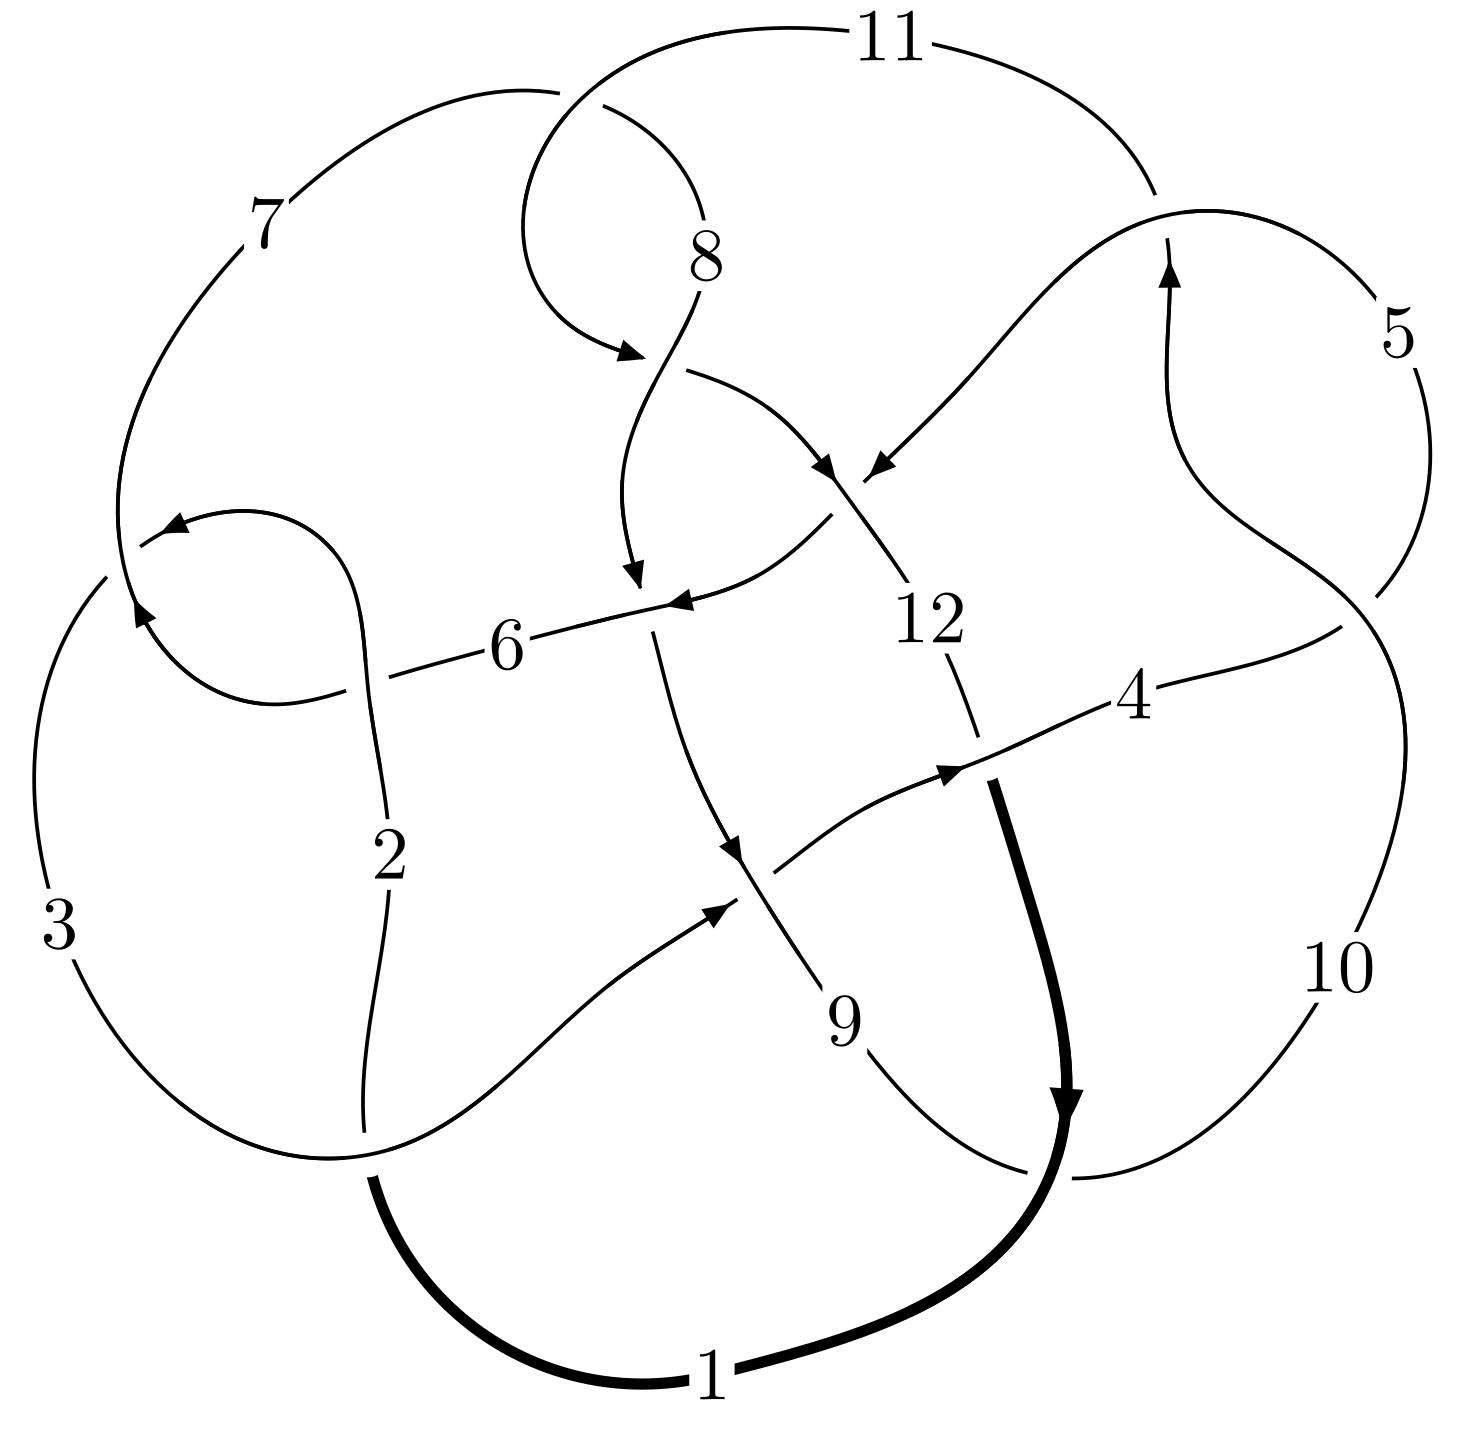
\includegraphics[width=112pt]{../../../GIT/diagram.site/Diagrams/png/1389_12a_0588.png}\\
\ \ \ A knot diagram\footnotemark}&
\allowdisplaybreaks
\textbf{Linearized knot diagam} \\
\cline{2-2}
 &
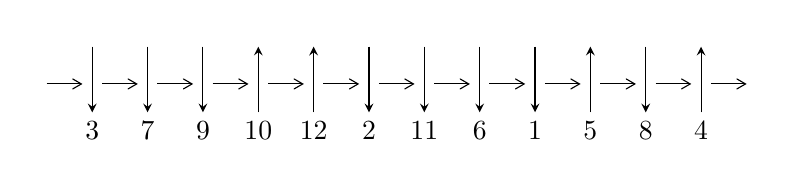
\begin{tikzpicture}[x=20pt, y=17pt]
	% nodes
	\node (C0) at (0, 0) {};
	\node (C1) at (1, 0) {};
	\node (C1U) at (1, +1) {};
	\node (C1D) at (1, -1) {3};

	\node (C2) at (2, 0) {};
	\node (C2U) at (2, +1) {};
	\node (C2D) at (2, -1) {7};

	\node (C3) at (3, 0) {};
	\node (C3U) at (3, +1) {};
	\node (C3D) at (3, -1) {9};

	\node (C4) at (4, 0) {};
	\node (C4U) at (4, +1) {};
	\node (C4D) at (4, -1) {10};

	\node (C5) at (5, 0) {};
	\node (C5U) at (5, +1) {};
	\node (C5D) at (5, -1) {12};

	\node (C6) at (6, 0) {};
	\node (C6U) at (6, +1) {};
	\node (C6D) at (6, -1) {2};

	\node (C7) at (7, 0) {};
	\node (C7U) at (7, +1) {};
	\node (C7D) at (7, -1) {11};

	\node (C8) at (8, 0) {};
	\node (C8U) at (8, +1) {};
	\node (C8D) at (8, -1) {6};

	\node (C9) at (9, 0) {};
	\node (C9U) at (9, +1) {};
	\node (C9D) at (9, -1) {1};

	\node (C10) at (10, 0) {};
	\node (C10U) at (10, +1) {};
	\node (C10D) at (10, -1) {5};

	\node (C11) at (11, 0) {};
	\node (C11U) at (11, +1) {};
	\node (C11D) at (11, -1) {8};

	\node (C12) at (12, 0) {};
	\node (C12U) at (12, +1) {};
	\node (C12D) at (12, -1) {4};
	\node (C13) at (13, 0) {};

	% arrows
	\draw[->,>={angle 60}]
	(C0) edge (C1) (C1) edge (C2) (C2) edge (C3) (C3) edge (C4) (C4) edge (C5) (C5) edge (C6) (C6) edge (C7) (C7) edge (C8) (C8) edge (C9) (C9) edge (C10) (C10) edge (C11) (C11) edge (C12) (C12) edge (C13) ;	\draw[->,>=stealth]
	(C1U) edge (C1D) (C2U) edge (C2D) (C3U) edge (C3D) (C4D) edge (C4U) (C5D) edge (C5U) (C6U) edge (C6D) (C7U) edge (C7D) (C8U) edge (C8D) (C9U) edge (C9D) (C10D) edge (C10U) (C11U) edge (C11D) (C12D) edge (C12U) ;
	\end{tikzpicture} \\
\hhline{~~} \\& 
\textbf{Solving Sequence} \\ \cline{2-2} 
 &
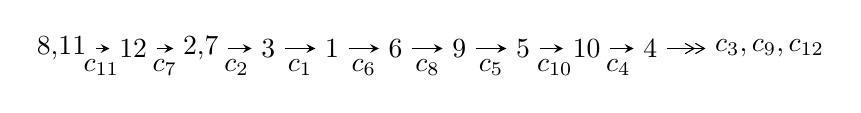
\begin{tikzpicture}[x=23pt, y=7pt]
	% node
	\node (A0) at (-1/8, 0) {8,11};
	\node (A1) at (1, 0) {12};
	\node (A2) at (33/16, 0) {2,7};
	\node (A3) at (25/8, 0) {3};
	\node (A4) at (33/8, 0) {1};
	\node (A5) at (41/8, 0) {6};
	\node (A6) at (49/8, 0) {9};
	\node (A7) at (57/8, 0) {5};
	\node (A8) at (65/8, 0) {10};
	\node (A9) at (73/8, 0) {4};
	\node (C1) at (1/2, -1) {$c_{11}$};
	\node (C2) at (3/2, -1) {$c_{7}$};
	\node (C3) at (21/8, -1) {$c_{2}$};
	\node (C4) at (29/8, -1) {$c_{1}$};
	\node (C5) at (37/8, -1) {$c_{6}$};
	\node (C6) at (45/8, -1) {$c_{8}$};
	\node (C7) at (53/8, -1) {$c_{5}$};
	\node (C8) at (61/8, -1) {$c_{10}$};
	\node (C9) at (69/8, -1) {$c_{4}$};
	\node (A10) at (11, 0) {$c_{3},c_{9},c_{12}$};

	% edge
	\draw[->,>=stealth]	
	(A0) edge (A1) (A1) edge (A2) (A2) edge (A3) (A3) edge (A4) (A4) edge (A5) (A5) edge (A6) (A6) edge (A7) (A7) edge (A8) (A8) edge (A9) ;
	\draw[->>,>={angle 60}]	
	(A9) edge (A10);
\end{tikzpicture} \\ 

\end{tabular} \\

\footnotetext{
The image of knot diagram is generated by the software ``\textbf{Draw programme}" developed by Andrew Bartholomew(\url{http://www.layer8.co.uk/maths/draw/index.htm\#Running-draw}), where we modified some parts for our purpose(\url{https://github.com/CATsTAILs/LinksPainter}).
}\phantom \\ \newline 
\centering \textbf{Ideals for irreducible components\footnotemark of $X_{\text{par}}$} 
 
\begin{align*}
I^u_{1}&=\langle 
-7.06111\times10^{773} u^{166}+1.98874\times10^{774} u^{165}+\cdots+4.70005\times10^{772} b-5.06349\times10^{777},\\
\phantom{I^u_{1}}&\phantom{= \langle  }-2.89028\times10^{777} u^{166}+8.09192\times10^{777} u^{165}+\cdots+2.74812\times10^{776} a-2.11200\times10^{781},\\
\phantom{I^u_{1}}&\phantom{= \langle  }u^{167}-2 u^{166}+\cdots+46140 u+5847\rangle \\
I^u_{2}&=\langle 
9.18102\times10^{17} u^{38}-1.34409\times10^{19} u^{37}+\cdots+9.06237\times10^{15} b-3.91149\times10^{19},\\
\phantom{I^u_{2}}&\phantom{= \langle  }-1.28417\times10^{19} u^{38}+4.98704\times10^{19} u^{37}+\cdots+9.06237\times10^{15} a-3.71425\times10^{18},\;u^{39}-5 u^{38}+\cdots-9 u+1\rangle \\
I^u_{3}&=\langle 
b- a-1,\;a^2-3 a+1,\;u+1\rangle \\
\\
I^v_{1}&=\langle 
a,\;b+1,\;v-1\rangle \\
\end{align*}
\raggedright * 4 irreducible components of $\dim_{\mathbb{C}}=0$, with total 209 representations.\\
\footnotetext{All coefficients of polynomials are rational numbers. But the coefficients are sometimes approximated in decimal forms when there is not enough margin.}
\newpage
\renewcommand{\arraystretch}{1}
\centering \section*{I. $I^u_{1}= \langle -7.06\times10^{773} u^{166}+1.99\times10^{774} u^{165}+\cdots+4.70\times10^{772} b-5.06\times10^{777},\;-2.89\times10^{777} u^{166}+8.09\times10^{777} u^{165}+\cdots+2.75\times10^{776} a-2.11\times10^{781},\;u^{167}-2 u^{166}+\cdots+46140 u+5847 \rangle$}
\flushleft \textbf{(i) Arc colorings}\\
\begin{tabular}{m{7pt} m{180pt} m{7pt} m{180pt} }
\flushright $a_{8}=$&$\begin{pmatrix}0\\u\end{pmatrix}$ \\
\flushright $a_{11}=$&$\begin{pmatrix}1\\0\end{pmatrix}$ \\
\flushright $a_{12}=$&$\begin{pmatrix}1\\u^2\end{pmatrix}$ \\
\flushright $a_{2}=$&$\begin{pmatrix}10.5173 u^{166}-29.4453 u^{165}+\cdots+510485. u+76852.5\\15.0235 u^{166}-42.3132 u^{165}+\cdots+717941. u+107733.\end{pmatrix}$ \\
\flushright $a_{7}=$&$\begin{pmatrix}u\\u\end{pmatrix}$ \\
\flushright $a_{3}=$&$\begin{pmatrix}7.22247 u^{166}-20.0391 u^{165}+\cdots+358938. u+54309.3\\11.7287 u^{166}-32.9070 u^{165}+\cdots+566395. u+85189.5\end{pmatrix}$ \\
\flushright $a_{1}=$&$\begin{pmatrix}39.2230 u^{166}-111.042 u^{165}+\cdots+1.84559\times10^{6} u+275964.\\18.7469 u^{166}-53.1149 u^{165}+\cdots+880172. u+131530.\end{pmatrix}$ \\
\flushright $a_{6}=$&$\begin{pmatrix}0.661216 u^{166}-2.29430 u^{165}+\cdots+11316.9 u+1043.92\\-12.4536 u^{166}+34.9983 u^{165}+\cdots-598548. u-89946.7\end{pmatrix}$ \\
\flushright $a_{9}=$&$\begin{pmatrix}-79.9532 u^{166}+226.459 u^{165}+\cdots-3.75759\times10^{6} u-561688.\\-57.9512 u^{166}+164.085 u^{165}+\cdots-2.72593\times10^{6} u-407523.\end{pmatrix}$ \\
\flushright $a_{5}=$&$\begin{pmatrix}14.2566 u^{166}-40.7929 u^{165}+\cdots+650841. u+96673.1\\-3.04496 u^{166}+8.35531 u^{165}+\cdots-156295. u-23829.6\end{pmatrix}$ \\
\flushright $a_{10}=$&$\begin{pmatrix}-53.0429 u^{166}+150.311 u^{165}+\cdots-2.48802\times10^{6} u-371738.\\-51.4081 u^{166}+145.510 u^{165}+\cdots-2.41953\times10^{6} u-361765.\end{pmatrix}$ \\
\flushright $a_{4}=$&$\begin{pmatrix}-6.89637 u^{166}+16.0888 u^{165}+\cdots-483395. u-77477.5\\6.82176 u^{166}-21.7442 u^{165}+\cdots+209405. u+27717.5\end{pmatrix}$\\&\end{tabular}
\flushleft \textbf{(ii) Obstruction class $= -1$}\\~\\
\flushleft \textbf{(iii) Cusp Shapes $= -1337.96 u^{166}+3790.87 u^{165}+\cdots-6.28006\times10^{7} u-9.38419\times10^{6}$}\\~\\
\newpage\renewcommand{\arraystretch}{1}
\flushleft \textbf{(iv) u-Polynomials at the component}\newline \\
\begin{tabular}{m{50pt}|m{274pt}}
Crossings & \hspace{64pt}u-Polynomials at each crossing \\
\hline $$\begin{aligned}c_{1}\end{aligned}$$&$\begin{aligned}
&u^{167}+71 u^{166}+\cdots+2794905 u+88209
\end{aligned}$\\
\hline $$\begin{aligned}c_{2},c_{6}\end{aligned}$$&$\begin{aligned}
&u^{167}-3 u^{166}+\cdots-1611 u-297
\end{aligned}$\\
\hline $$\begin{aligned}c_{3}\end{aligned}$$&$\begin{aligned}
&u^{167}- u^{166}+\cdots+9 u-1
\end{aligned}$\\
\hline $$\begin{aligned}c_{4},c_{10}\end{aligned}$$&$\begin{aligned}
&u^{167}+u^{166}+\cdots+286094 u+26963
\end{aligned}$\\
\hline $$\begin{aligned}c_{5}\end{aligned}$$&$\begin{aligned}
&u^{167}-4 u^{166}+\cdots-98117 u+118061
\end{aligned}$\\
\hline $$\begin{aligned}c_{7},c_{11}\end{aligned}$$&$\begin{aligned}
&u^{167}-2 u^{166}+\cdots+46140 u+5847
\end{aligned}$\\
\hline $$\begin{aligned}c_{8}\end{aligned}$$&$\begin{aligned}
&u^{167}-5 u^{166}+\cdots-30593750 u+2687500
\end{aligned}$\\
\hline $$\begin{aligned}c_{9}\end{aligned}$$&$\begin{aligned}
&u^{167}+9 u^{166}+\cdots-1286138 u-711596
\end{aligned}$\\
\hline $$\begin{aligned}c_{12}\end{aligned}$$&$\begin{aligned}
&u^{167}+17 u^{166}+\cdots-36 u-12
\end{aligned}$\\
\hline
\end{tabular}\\~\\
\newpage\renewcommand{\arraystretch}{1}
\flushleft \textbf{(v) Riley Polynomials at the component}\newline \\
\begin{tabular}{m{50pt}|m{274pt}}
Crossings & \hspace{64pt}Riley Polynomials at each crossing \\
\hline $$\begin{aligned}c_{1}\end{aligned}$$&$\begin{aligned}
&y^{167}+53 y^{166}+\cdots-16946980639767 y-7780827681
\end{aligned}$\\
\hline $$\begin{aligned}c_{2},c_{6}\end{aligned}$$&$\begin{aligned}
&y^{167}-71 y^{166}+\cdots+2794905 y-88209
\end{aligned}$\\
\hline $$\begin{aligned}c_{3}\end{aligned}$$&$\begin{aligned}
&y^{167}+19 y^{166}+\cdots+903 y-1
\end{aligned}$\\
\hline $$\begin{aligned}c_{4},c_{10}\end{aligned}$$&$\begin{aligned}
&y^{167}-109 y^{166}+\cdots+67092980862 y-727003369
\end{aligned}$\\
\hline $$\begin{aligned}c_{5}\end{aligned}$$&$\begin{aligned}
&y^{167}+16 y^{166}+\cdots-734586387985 y-13938399721
\end{aligned}$\\
\hline $$\begin{aligned}c_{7},c_{11}\end{aligned}$$&$\begin{aligned}
&y^{167}-86 y^{166}+\cdots+1156461642 y-34187409
\end{aligned}$\\
\hline $$\begin{aligned}c_{8}\end{aligned}$$&$\begin{aligned}
&y^{167}-17 y^{166}+\cdots+606399335937500 y-7222656250000
\end{aligned}$\\
\hline $$\begin{aligned}c_{9}\end{aligned}$$&$\begin{aligned}
&y^{167}+55 y^{166}+\cdots-11009677597860 y-506368867216
\end{aligned}$\\
\hline $$\begin{aligned}c_{12}\end{aligned}$$&$\begin{aligned}
&y^{167}-29 y^{166}+\cdots+6408 y-144
\end{aligned}$\\
\hline
\end{tabular}\\~\\
\newpage\flushleft \textbf{(vi) Complex Volumes and Cusp Shapes}
$$\begin{array}{c|c|c}  
\text{Solutions to }I^u_{1}& \I (\text{vol} + \sqrt{-1}CS) & \text{Cusp shape}\\
 \hline 
\begin{aligned}
u &= -0.972662 + 0.230057 I \\
a &= -0.714704 + 0.054338 I \\
b &= -0.629457 + 0.206535 I\end{aligned}
 & -1.74998 + 0.43329 I & \phantom{-0.000000 } 0 \\ \hline\begin{aligned}
u &= -0.972662 - 0.230057 I \\
a &= -0.714704 - 0.054338 I \\
b &= -0.629457 - 0.206535 I\end{aligned}
 & -1.74998 - 0.43329 I & \phantom{-0.000000 } 0 \\ \hline\begin{aligned}
u &= \phantom{-}0.821125 + 0.560089 I \\
a &= \phantom{-}0.457294 - 0.470633 I \\
b &= \phantom{-}1.66147 - 0.32360 I\end{aligned}
 & \phantom{-}4.79609 - 5.26583 I & \phantom{-0.000000 } 0 \\ \hline\begin{aligned}
u &= \phantom{-}0.821125 - 0.560089 I \\
a &= \phantom{-}0.457294 + 0.470633 I \\
b &= \phantom{-}1.66147 + 0.32360 I\end{aligned}
 & \phantom{-}4.79609 + 5.26583 I & \phantom{-0.000000 } 0 \\ \hline\begin{aligned}
u &= \phantom{-}0.039794 + 0.986024 I \\
a &= \phantom{-}0.18398 - 1.64651 I \\
b &= \phantom{-}0.817154 - 0.578261 I\end{aligned}
 & \phantom{-}0.11929 + 8.53958 I & \phantom{-0.000000 } 0 \\ \hline\begin{aligned}
u &= \phantom{-}0.039794 - 0.986024 I \\
a &= \phantom{-}0.18398 + 1.64651 I \\
b &= \phantom{-}0.817154 + 0.578261 I\end{aligned}
 & \phantom{-}0.11929 - 8.53958 I & \phantom{-0.000000 } 0 \\ \hline\begin{aligned}
u &= -0.894406 + 0.414575 I \\
a &= -0.467639 + 0.689638 I \\
b &= \phantom{-}0.505608 + 0.092764 I\end{aligned}
 & \phantom{-}5.21083 - 0.90333 I & \phantom{-0.000000 } 0 \\ \hline\begin{aligned}
u &= -0.894406 - 0.414575 I \\
a &= -0.467639 - 0.689638 I \\
b &= \phantom{-}0.505608 - 0.092764 I\end{aligned}
 & \phantom{-}5.21083 + 0.90333 I & \phantom{-0.000000 } 0 \\ \hline\begin{aligned}
u &= \phantom{-}0.801414 + 0.625750 I \\
a &= -0.474913 + 0.949506 I \\
b &= -0.261128 - 0.222516 I\end{aligned}
 & \phantom{-}4.85064 + 0.68988 I & \phantom{-0.000000 } 0 \\ \hline\begin{aligned}
u &= \phantom{-}0.801414 - 0.625750 I \\
a &= -0.474913 - 0.949506 I \\
b &= -0.261128 + 0.222516 I\end{aligned}
 & \phantom{-}4.85064 - 0.68988 I & \phantom{-0.000000 } 0\\
 \hline 
 \end{array}$$\newpage$$\begin{array}{c|c|c}  
\text{Solutions to }I^u_{1}& \I (\text{vol} + \sqrt{-1}CS) & \text{Cusp shape}\\
 \hline 
\begin{aligned}
u &= -0.942240 + 0.252531 I \\
a &= -1.13569 - 1.23380 I \\
b &= -2.34372 - 0.69387 I\end{aligned}
 & \phantom{-}2.20316 + 4.25845 I & \phantom{-0.000000 } 0 \\ \hline\begin{aligned}
u &= -0.942240 - 0.252531 I \\
a &= -1.13569 + 1.23380 I \\
b &= -2.34372 + 0.69387 I\end{aligned}
 & \phantom{-}2.20316 - 4.25845 I & \phantom{-0.000000 } 0 \\ \hline\begin{aligned}
u &= \phantom{-}0.864699 + 0.448507 I \\
a &= \phantom{-}0.57238 + 1.37555 I \\
b &= -0.606818 + 1.182450 I\end{aligned}
 & \phantom{-}4.25327 - 10.46020 I & \phantom{-0.000000 } 0 \\ \hline\begin{aligned}
u &= \phantom{-}0.864699 - 0.448507 I \\
a &= \phantom{-}0.57238 - 1.37555 I \\
b &= -0.606818 - 1.182450 I\end{aligned}
 & \phantom{-}4.25327 + 10.46020 I & \phantom{-0.000000 } 0 \\ \hline\begin{aligned}
u &= \phantom{-}0.872923 + 0.539032 I \\
a &= -0.028634 - 0.661713 I \\
b &= -0.814435 - 0.686233 I\end{aligned}
 & -2.00357 - 3.87173 I & \phantom{-0.000000 } 0 \\ \hline\begin{aligned}
u &= \phantom{-}0.872923 - 0.539032 I \\
a &= -0.028634 + 0.661713 I \\
b &= -0.814435 + 0.686233 I\end{aligned}
 & -2.00357 + 3.87173 I & \phantom{-0.000000 } 0 \\ \hline\begin{aligned}
u &= \phantom{-}0.764718 + 0.593333 I \\
a &= -0.224352 + 0.611378 I \\
b &= \phantom{-}0.003174 - 0.502837 I\end{aligned}
 & \phantom{-}4.86027 + 0.57727 I & \phantom{-0.000000 } 0 \\ \hline\begin{aligned}
u &= \phantom{-}0.764718 - 0.593333 I \\
a &= -0.224352 - 0.611378 I \\
b &= \phantom{-}0.003174 + 0.502837 I\end{aligned}
 & \phantom{-}4.86027 - 0.57727 I & \phantom{-0.000000 } 0 \\ \hline\begin{aligned}
u &= \phantom{-}0.807662 + 0.525764 I \\
a &= -0.109429 - 0.467702 I \\
b &= \phantom{-}1.103770 - 0.284116 I\end{aligned}
 & \phantom{-}4.72818 - 5.02734 I & \phantom{-0.000000 } 0 \\ \hline\begin{aligned}
u &= \phantom{-}0.807662 - 0.525764 I \\
a &= -0.109429 + 0.467702 I \\
b &= \phantom{-}1.103770 + 0.284116 I\end{aligned}
 & \phantom{-}4.72818 + 5.02734 I & \phantom{-0.000000 } 0\\
 \hline 
 \end{array}$$\newpage$$\begin{array}{c|c|c}  
\text{Solutions to }I^u_{1}& \I (\text{vol} + \sqrt{-1}CS) & \text{Cusp shape}\\
 \hline 
\begin{aligned}
u &= -1.03726\phantom{ +0.000000I} \\
a &= \phantom{-}3.68109\phantom{ +0.000000I} \\
b &= \phantom{-}4.54373\phantom{ +0.000000I}\end{aligned}
 & -3.13749\phantom{ +0.000000I} & \phantom{-0.000000 } 0 \\ \hline\begin{aligned}
u &= -0.897317 + 0.347194 I \\
a &= \phantom{-}1.41904 - 0.00440 I \\
b &= \phantom{-}2.79934 - 0.20867 I\end{aligned}
 & \phantom{-}3.47117 + 10.13850 I & \phantom{-0.000000 } 0 \\ \hline\begin{aligned}
u &= -0.897317 - 0.347194 I \\
a &= \phantom{-}1.41904 + 0.00440 I \\
b &= \phantom{-}2.79934 + 0.20867 I\end{aligned}
 & \phantom{-}3.47117 - 10.13850 I & \phantom{-0.000000 } 0 \\ \hline\begin{aligned}
u &= \phantom{-}1.018550 + 0.259841 I \\
a &= \phantom{-}0.071552 + 0.245607 I \\
b &= -0.609424 - 0.451865 I\end{aligned}
 & -2.58602 - 3.93355 I & \phantom{-0.000000 } 0 \\ \hline\begin{aligned}
u &= \phantom{-}1.018550 - 0.259841 I \\
a &= \phantom{-}0.071552 - 0.245607 I \\
b &= -0.609424 + 0.451865 I\end{aligned}
 & -2.58602 + 3.93355 I & \phantom{-0.000000 } 0 \\ \hline\begin{aligned}
u &= \phantom{-}0.878831 + 0.341393 I \\
a &= \phantom{-}1.05330 - 2.00228 I \\
b &= \phantom{-}0.565038 - 0.965512 I\end{aligned}
 & \phantom{-}4.72304 - 4.97410 I & \phantom{-0.000000 } 0 \\ \hline\begin{aligned}
u &= \phantom{-}0.878831 - 0.341393 I \\
a &= \phantom{-}1.05330 + 2.00228 I \\
b &= \phantom{-}0.565038 + 0.965512 I\end{aligned}
 & \phantom{-}4.72304 + 4.97410 I & \phantom{-0.000000 } 0 \\ \hline\begin{aligned}
u &= -1.025650 + 0.269556 I \\
a &= -2.30755 + 0.91685 I \\
b &= -3.16643 + 0.41485 I\end{aligned}
 & -5.43574 + 0.32299 I & \phantom{-0.000000 } 0 \\ \hline\begin{aligned}
u &= -1.025650 - 0.269556 I \\
a &= -2.30755 - 0.91685 I \\
b &= -3.16643 - 0.41485 I\end{aligned}
 & -5.43574 - 0.32299 I & \phantom{-0.000000 } 0 \\ \hline\begin{aligned}
u &= \phantom{-}0.777394 + 0.493312 I \\
a &= \phantom{-}0.720123 + 0.423177 I \\
b &= \phantom{-}0.20264 + 1.47698 I\end{aligned}
 & \phantom{-}4.51945 + 6.57191 I & \phantom{-0.000000 } 0\\
 \hline 
 \end{array}$$\newpage$$\begin{array}{c|c|c}  
\text{Solutions to }I^u_{1}& \I (\text{vol} + \sqrt{-1}CS) & \text{Cusp shape}\\
 \hline 
\begin{aligned}
u &= \phantom{-}0.777394 - 0.493312 I \\
a &= \phantom{-}0.720123 - 0.423177 I \\
b &= \phantom{-}0.20264 - 1.47698 I\end{aligned}
 & \phantom{-}4.51945 - 6.57191 I & \phantom{-0.000000 } 0 \\ \hline\begin{aligned}
u &= \phantom{-}0.187205 + 0.889090 I \\
a &= \phantom{-}0.03570 + 2.05620 I \\
b &= -0.330273 + 0.835028 I\end{aligned}
 & \phantom{-}0.92581 + 6.07862 I & \phantom{-0.000000 } 0 \\ \hline\begin{aligned}
u &= \phantom{-}0.187205 - 0.889090 I \\
a &= \phantom{-}0.03570 - 2.05620 I \\
b &= -0.330273 - 0.835028 I\end{aligned}
 & \phantom{-}0.92581 - 6.07862 I & \phantom{-0.000000 } 0 \\ \hline\begin{aligned}
u &= -0.021949 + 1.093140 I \\
a &= \phantom{-}0.26200 - 1.66572 I \\
b &= \phantom{-}0.270816 - 0.551047 I\end{aligned}
 & -0.45503 - 6.15957 I & \phantom{-0.000000 } 0 \\ \hline\begin{aligned}
u &= -0.021949 - 1.093140 I \\
a &= \phantom{-}0.26200 + 1.66572 I \\
b &= \phantom{-}0.270816 + 0.551047 I\end{aligned}
 & -0.45503 + 6.15957 I & \phantom{-0.000000 } 0 \\ \hline\begin{aligned}
u &= \phantom{-}0.765199 + 0.480119 I \\
a &= -0.33579 + 1.43118 I \\
b &= -0.005294 + 0.173701 I\end{aligned}
 & \phantom{-}4.82252 + 0.90757 I & \phantom{-0.000000 } 0 \\ \hline\begin{aligned}
u &= \phantom{-}0.765199 - 0.480119 I \\
a &= -0.33579 - 1.43118 I \\
b &= -0.005294 - 0.173701 I\end{aligned}
 & \phantom{-}4.82252 - 0.90757 I & \phantom{-0.000000 } 0 \\ \hline\begin{aligned}
u &= -1.016800 + 0.443199 I \\
a &= -0.644176 + 0.375189 I \\
b &= -0.369034 + 1.056070 I\end{aligned}
 & -2.16138 + 1.67808 I & \phantom{-0.000000 } 0 \\ \hline\begin{aligned}
u &= -1.016800 - 0.443199 I \\
a &= -0.644176 - 0.375189 I \\
b &= -0.369034 - 1.056070 I\end{aligned}
 & -2.16138 - 1.67808 I & \phantom{-0.000000 } 0 \\ \hline\begin{aligned}
u &= -0.351162 + 1.053340 I \\
a &= -0.0276257 + 0.1218040 I \\
b &= -0.935297 - 0.078163 I\end{aligned}
 & \phantom{-}6.01572 - 8.10134 I & \phantom{-0.000000 } 0\\
 \hline 
 \end{array}$$\newpage$$\begin{array}{c|c|c}  
\text{Solutions to }I^u_{1}& \I (\text{vol} + \sqrt{-1}CS) & \text{Cusp shape}\\
 \hline 
\begin{aligned}
u &= -0.351162 - 1.053340 I \\
a &= -0.0276257 - 0.1218040 I \\
b &= -0.935297 + 0.078163 I\end{aligned}
 & \phantom{-}6.01572 + 8.10134 I & \phantom{-0.000000 } 0 \\ \hline\begin{aligned}
u &= -0.852820 + 0.226205 I \\
a &= \phantom{-}1.019270 + 0.598571 I \\
b &= \phantom{-}0.292599 - 0.596293 I\end{aligned}
 & \phantom{-}2.55823 - 2.10130 I & \phantom{-0.000000 } 0 \\ \hline\begin{aligned}
u &= -0.852820 - 0.226205 I \\
a &= \phantom{-}1.019270 - 0.598571 I \\
b &= \phantom{-}0.292599 + 0.596293 I\end{aligned}
 & \phantom{-}2.55823 + 2.10130 I & \phantom{-0.000000 } 0 \\ \hline\begin{aligned}
u &= \phantom{-}1.122420 + 0.040813 I \\
a &= -1.050590 - 0.673726 I \\
b &= -2.09129 - 0.10135 I\end{aligned}
 & -4.84462 + 2.01205 I & \phantom{-0.000000 } 0 \\ \hline\begin{aligned}
u &= \phantom{-}1.122420 - 0.040813 I \\
a &= -1.050590 + 0.673726 I \\
b &= -2.09129 + 0.10135 I\end{aligned}
 & -4.84462 - 2.01205 I & \phantom{-0.000000 } 0 \\ \hline\begin{aligned}
u &= \phantom{-}0.398803 + 0.780172 I \\
a &= -0.676907 + 0.558220 I \\
b &= -0.0453966 - 0.1333240 I\end{aligned}
 & \phantom{-}2.71184 + 2.00711 I & \phantom{-0.000000 } 0 \\ \hline\begin{aligned}
u &= \phantom{-}0.398803 - 0.780172 I \\
a &= -0.676907 - 0.558220 I \\
b &= -0.0453966 + 0.1333240 I\end{aligned}
 & \phantom{-}2.71184 - 2.00711 I & \phantom{-0.000000 } 0 \\ \hline\begin{aligned}
u &= \phantom{-}0.824347 + 0.289882 I \\
a &= -2.62081 + 0.89290 I \\
b &= -3.67138 + 0.60920 I\end{aligned}
 & \phantom{-}4.99211 + 2.13455 I & \phantom{-0.000000 } 0 \\ \hline\begin{aligned}
u &= \phantom{-}0.824347 - 0.289882 I \\
a &= -2.62081 - 0.89290 I \\
b &= -3.67138 - 0.60920 I\end{aligned}
 & \phantom{-}4.99211 - 2.13455 I & \phantom{-0.000000 } 0 \\ \hline\begin{aligned}
u &= \phantom{-}0.092978 + 0.867549 I \\
a &= \phantom{-}0.314473 - 0.607042 I \\
b &= -0.627542 + 0.003275 I\end{aligned}
 & \phantom{-}1.35564 + 3.10692 I & \phantom{-0.000000 } 0\\
 \hline 
 \end{array}$$\newpage$$\begin{array}{c|c|c}  
\text{Solutions to }I^u_{1}& \I (\text{vol} + \sqrt{-1}CS) & \text{Cusp shape}\\
 \hline 
\begin{aligned}
u &= \phantom{-}0.092978 - 0.867549 I \\
a &= \phantom{-}0.314473 + 0.607042 I \\
b &= -0.627542 - 0.003275 I\end{aligned}
 & \phantom{-}1.35564 - 3.10692 I & \phantom{-0.000000 } 0 \\ \hline\begin{aligned}
u &= -0.792901 + 0.355099 I \\
a &= -0.26167 - 1.82672 I \\
b &= \phantom{-}0.518383 - 0.533921 I\end{aligned}
 & \phantom{-}3.80719 - 7.07343 I & \phantom{-0.000000 } 0 \\ \hline\begin{aligned}
u &= -0.792901 - 0.355099 I \\
a &= -0.26167 + 1.82672 I \\
b &= \phantom{-}0.518383 + 0.533921 I\end{aligned}
 & \phantom{-}3.80719 + 7.07343 I & \phantom{-0.000000 } 0 \\ \hline\begin{aligned}
u &= -0.788640 + 0.339798 I \\
a &= -1.47249 - 0.51463 I \\
b &= -0.895767 + 0.050514 I\end{aligned}
 & -1.85499 + 0.29361 I & \phantom{-0.000000 } 0 \\ \hline\begin{aligned}
u &= -0.788640 - 0.339798 I \\
a &= -1.47249 + 0.51463 I \\
b &= -0.895767 - 0.050514 I\end{aligned}
 & -1.85499 - 0.29361 I & \phantom{-0.000000 } 0 \\ \hline\begin{aligned}
u &= \phantom{-}1.091310 + 0.405083 I \\
a &= -0.001384 + 0.328024 I \\
b &= \phantom{-}0.018709 - 0.539674 I\end{aligned}
 & \phantom{-}0.86485 - 3.58498 I & \phantom{-0.000000 } 0 \\ \hline\begin{aligned}
u &= \phantom{-}1.091310 - 0.405083 I \\
a &= -0.001384 - 0.328024 I \\
b &= \phantom{-}0.018709 + 0.539674 I\end{aligned}
 & \phantom{-}0.86485 + 3.58498 I & \phantom{-0.000000 } 0 \\ \hline\begin{aligned}
u &= -1.087430 + 0.415532 I \\
a &= -0.128643 - 0.308564 I \\
b &= -0.597632 - 0.988389 I\end{aligned}
 & -0.912275 - 0.937931 I & \phantom{-0.000000 } 0 \\ \hline\begin{aligned}
u &= -1.087430 - 0.415532 I \\
a &= -0.128643 + 0.308564 I \\
b &= -0.597632 + 0.988389 I\end{aligned}
 & -0.912275 + 0.937931 I & \phantom{-0.000000 } 0 \\ \hline\begin{aligned}
u &= -0.724392 + 0.412992 I \\
a &= \phantom{-}1.12167 + 1.41576 I \\
b &= \phantom{-}0.248043 + 1.093250 I\end{aligned}
 & -4.11167 + 2.24501 I & \phantom{-0.000000 } 0\\
 \hline 
 \end{array}$$\newpage$$\begin{array}{c|c|c}  
\text{Solutions to }I^u_{1}& \I (\text{vol} + \sqrt{-1}CS) & \text{Cusp shape}\\
 \hline 
\begin{aligned}
u &= -0.724392 - 0.412992 I \\
a &= \phantom{-}1.12167 - 1.41576 I \\
b &= \phantom{-}0.248043 - 1.093250 I\end{aligned}
 & -4.11167 - 2.24501 I & \phantom{-0.000000 } 0 \\ \hline\begin{aligned}
u &= -0.831820 + 0.017037 I \\
a &= \phantom{-}2.33554 - 3.06965 I \\
b &= \phantom{-}1.26334 - 2.18652 I\end{aligned}
 & \phantom{-}1.81851 + 2.85219 I & \phantom{-0.000000 } 0 \\ \hline\begin{aligned}
u &= -0.831820 - 0.017037 I \\
a &= \phantom{-}2.33554 + 3.06965 I \\
b &= \phantom{-}1.26334 + 2.18652 I\end{aligned}
 & \phantom{-}1.81851 - 2.85219 I & \phantom{-0.000000 } 0 \\ \hline\begin{aligned}
u &= \phantom{-}0.344357 + 0.753523 I \\
a &= -0.492546 + 0.258225 I \\
b &= \phantom{-}0.282513 + 0.131141 I\end{aligned}
 & \phantom{-}2.55307 + 1.66800 I & \phantom{-0.000000 } 0 \\ \hline\begin{aligned}
u &= \phantom{-}0.344357 - 0.753523 I \\
a &= -0.492546 - 0.258225 I \\
b &= \phantom{-}0.282513 - 0.131141 I\end{aligned}
 & \phantom{-}2.55307 - 1.66800 I & \phantom{-0.000000 } 0 \\ \hline\begin{aligned}
u &= \phantom{-}1.095270 + 0.416653 I \\
a &= -1.54064 - 0.99695 I \\
b &= -2.42748 - 0.40304 I\end{aligned}
 & -4.08354 - 3.20236 I & \phantom{-0.000000 } 0 \\ \hline\begin{aligned}
u &= \phantom{-}1.095270 - 0.416653 I \\
a &= -1.54064 + 0.99695 I \\
b &= -2.42748 + 0.40304 I\end{aligned}
 & -4.08354 + 3.20236 I & \phantom{-0.000000 } 0 \\ \hline\begin{aligned}
u &= -1.17213\phantom{ +0.000000I} \\
a &= -0.922587\phantom{ +0.000000I} \\
b &= -1.73912\phantom{ +0.000000I}\end{aligned}
 & -2.83879\phantom{ +0.000000I} & \phantom{-0.000000 } 0 \\ \hline\begin{aligned}
u &= -0.826385\phantom{ +0.000000I} \\
a &= -0.917377\phantom{ +0.000000I} \\
b &= -2.75477\phantom{ +0.000000I}\end{aligned}
 & -0.705957\phantom{ +0.000000I} & \phantom{-0.000000 } 0 \\ \hline\begin{aligned}
u &= -0.407511 + 1.106390 I \\
a &= \phantom{-}0.529226 - 0.143879 I \\
b &= \phantom{-}1.270910 - 0.032384 I\end{aligned}
 & \phantom{-}6.61099 + 1.46475 I & \phantom{-0.000000 } 0\\
 \hline 
 \end{array}$$\newpage$$\begin{array}{c|c|c}  
\text{Solutions to }I^u_{1}& \I (\text{vol} + \sqrt{-1}CS) & \text{Cusp shape}\\
 \hline 
\begin{aligned}
u &= -0.407511 - 1.106390 I \\
a &= \phantom{-}0.529226 + 0.143879 I \\
b &= \phantom{-}1.270910 + 0.032384 I\end{aligned}
 & \phantom{-}6.61099 - 1.46475 I & \phantom{-0.000000 } 0 \\ \hline\begin{aligned}
u &= -1.098180 + 0.447252 I \\
a &= \phantom{-}2.34715 + 0.76754 I \\
b &= \phantom{-}3.31921 + 0.63775 I\end{aligned}
 & -3.43399 + 6.32250 I & \phantom{-0.000000 } 0 \\ \hline\begin{aligned}
u &= -1.098180 - 0.447252 I \\
a &= \phantom{-}2.34715 - 0.76754 I \\
b &= \phantom{-}3.31921 - 0.63775 I\end{aligned}
 & -3.43399 - 6.32250 I & \phantom{-0.000000 } 0 \\ \hline\begin{aligned}
u &= -0.307719 + 0.745452 I \\
a &= \phantom{-}0.50216 + 1.92220 I \\
b &= \phantom{-}0.016544 + 0.780195 I\end{aligned}
 & -4.08290 + 2.57720 I & \phantom{-0.000000 } 0 \\ \hline\begin{aligned}
u &= -0.307719 - 0.745452 I \\
a &= \phantom{-}0.50216 - 1.92220 I \\
b &= \phantom{-}0.016544 - 0.780195 I\end{aligned}
 & -4.08290 - 2.57720 I & \phantom{-0.000000 } 0 \\ \hline\begin{aligned}
u &= -1.204090 + 0.039093 I \\
a &= \phantom{-}1.44148 + 1.52259 I \\
b &= \phantom{-}2.08490 + 1.30733 I\end{aligned}
 & -2.95281 + 0.67247 I & \phantom{-0.000000 } 0 \\ \hline\begin{aligned}
u &= -1.204090 - 0.039093 I \\
a &= \phantom{-}1.44148 - 1.52259 I \\
b &= \phantom{-}2.08490 - 1.30733 I\end{aligned}
 & -2.95281 - 0.67247 I & \phantom{-0.000000 } 0 \\ \hline\begin{aligned}
u &= \phantom{-}0.713714 + 0.342186 I \\
a &= \phantom{-}1.36260 - 1.29521 I \\
b &= \phantom{-}2.58306 - 0.99547 I\end{aligned}
 & \phantom{-}5.13802 - 4.71471 I & \phantom{-0.000000 } 0 \\ \hline\begin{aligned}
u &= \phantom{-}0.713714 - 0.342186 I \\
a &= \phantom{-}1.36260 + 1.29521 I \\
b &= \phantom{-}2.58306 + 0.99547 I\end{aligned}
 & \phantom{-}5.13802 + 4.71471 I & \phantom{-0.000000 } 0 \\ \hline\begin{aligned}
u &= \phantom{-}1.074270 + 0.570781 I \\
a &= -1.49456 - 0.84545 I \\
b &= -2.00878 - 0.22597 I\end{aligned}
 & -2.83698 - 0.68862 I & \phantom{-0.000000 } 0\\
 \hline 
 \end{array}$$\newpage$$\begin{array}{c|c|c}  
\text{Solutions to }I^u_{1}& \I (\text{vol} + \sqrt{-1}CS) & \text{Cusp shape}\\
 \hline 
\begin{aligned}
u &= \phantom{-}1.074270 - 0.570781 I \\
a &= -1.49456 + 0.84545 I \\
b &= -2.00878 + 0.22597 I\end{aligned}
 & -2.83698 + 0.68862 I & \phantom{-0.000000 } 0 \\ \hline\begin{aligned}
u &= -1.171690 + 0.339206 I \\
a &= \phantom{-}0.479015 + 0.777736 I \\
b &= \phantom{-}0.868747 + 0.476023 I\end{aligned}
 & -2.94382 + 0.96462 I & \phantom{-0.000000 } 0 \\ \hline\begin{aligned}
u &= -1.171690 - 0.339206 I \\
a &= \phantom{-}0.479015 - 0.777736 I \\
b &= \phantom{-}0.868747 - 0.476023 I\end{aligned}
 & -2.94382 - 0.96462 I & \phantom{-0.000000 } 0 \\ \hline\begin{aligned}
u &= -0.366444 + 1.164790 I \\
a &= \phantom{-}0.36161 + 1.76843 I \\
b &= \phantom{-}0.625432 + 0.738449 I\end{aligned}
 & \phantom{-}4.2665 - 13.9116 I & \phantom{-0.000000 } 0 \\ \hline\begin{aligned}
u &= -0.366444 - 1.164790 I \\
a &= \phantom{-}0.36161 - 1.76843 I \\
b &= \phantom{-}0.625432 - 0.738449 I\end{aligned}
 & \phantom{-}4.2665 + 13.9116 I & \phantom{-0.000000 } 0 \\ \hline\begin{aligned}
u &= \phantom{-}0.917100 + 0.807092 I \\
a &= -1.13593 + 1.11590 I \\
b &= -0.929625 + 0.348672 I\end{aligned}
 & -1.51643 - 0.92743 I & \phantom{-0.000000 } 0 \\ \hline\begin{aligned}
u &= \phantom{-}0.917100 - 0.807092 I \\
a &= -1.13593 - 1.11590 I \\
b &= -0.929625 - 0.348672 I\end{aligned}
 & -1.51643 + 0.92743 I & \phantom{-0.000000 } 0 \\ \hline\begin{aligned}
u &= -1.088940 + 0.560207 I \\
a &= \phantom{-}1.61092 + 0.88655 I \\
b &= \phantom{-}2.51985 + 0.90599 I\end{aligned}
 & -3.20452 + 3.95476 I & \phantom{-0.000000 } 0 \\ \hline\begin{aligned}
u &= -1.088940 - 0.560207 I \\
a &= \phantom{-}1.61092 - 0.88655 I \\
b &= \phantom{-}2.51985 - 0.90599 I\end{aligned}
 & -3.20452 - 3.95476 I & \phantom{-0.000000 } 0 \\ \hline\begin{aligned}
u &= -1.176440 + 0.365393 I \\
a &= -0.154254 - 0.460357 I \\
b &= -0.757170 + 0.469133 I\end{aligned}
 & \phantom{-}2.18325 + 7.21707 I & \phantom{-0.000000 } 0\\
 \hline 
 \end{array}$$\newpage$$\begin{array}{c|c|c}  
\text{Solutions to }I^u_{1}& \I (\text{vol} + \sqrt{-1}CS) & \text{Cusp shape}\\
 \hline 
\begin{aligned}
u &= -1.176440 - 0.365393 I \\
a &= -0.154254 + 0.460357 I \\
b &= -0.757170 - 0.469133 I\end{aligned}
 & \phantom{-}2.18325 - 7.21707 I & \phantom{-0.000000 } 0 \\ \hline\begin{aligned}
u &= -0.682130 + 0.352918 I \\
a &= \phantom{-}0.317815 - 0.020147 I \\
b &= \phantom{-}0.168107 + 1.249880 I\end{aligned}
 & \phantom{-}5.87369 + 4.34128 I & \phantom{-0.000000 } 0 \\ \hline\begin{aligned}
u &= -0.682130 - 0.352918 I \\
a &= \phantom{-}0.317815 + 0.020147 I \\
b &= \phantom{-}0.168107 - 1.249880 I\end{aligned}
 & \phantom{-}5.87369 - 4.34128 I & \phantom{-0.000000 } 0 \\ \hline\begin{aligned}
u &= \phantom{-}1.095280 + 0.579401 I \\
a &= \phantom{-}0.231558 - 0.424823 I \\
b &= \phantom{-}0.647454 - 0.755009 I\end{aligned}
 & \phantom{-}0.64781 - 7.09781 I & \phantom{-0.000000 } 0 \\ \hline\begin{aligned}
u &= \phantom{-}1.095280 - 0.579401 I \\
a &= \phantom{-}0.231558 + 0.424823 I \\
b &= \phantom{-}0.647454 + 0.755009 I\end{aligned}
 & \phantom{-}0.64781 + 7.09781 I & \phantom{-0.000000 } 0 \\ \hline\begin{aligned}
u &= \phantom{-}1.118200 + 0.548382 I \\
a &= -0.0060452 - 0.0355583 I \\
b &= -0.095778 - 0.615914 I\end{aligned}
 & \phantom{-}0.25306 - 6.57486 I & \phantom{-0.000000 } 0 \\ \hline\begin{aligned}
u &= \phantom{-}1.118200 - 0.548382 I \\
a &= -0.0060452 + 0.0355583 I \\
b &= -0.095778 + 0.615914 I\end{aligned}
 & \phantom{-}0.25306 + 6.57486 I & \phantom{-0.000000 } 0 \\ \hline\begin{aligned}
u &= -1.238610 + 0.271155 I \\
a &= -1.017820 + 0.563393 I \\
b &= -1.99341 + 0.13579 I\end{aligned}
 & -2.85298 + 0.64390 I & \phantom{-0.000000 } 0 \\ \hline\begin{aligned}
u &= -1.238610 - 0.271155 I \\
a &= -1.017820 - 0.563393 I \\
b &= -1.99341 - 0.13579 I\end{aligned}
 & -2.85298 - 0.64390 I & \phantom{-0.000000 } 0 \\ \hline\begin{aligned}
u &= -1.227170 + 0.344099 I \\
a &= -2.27737 - 0.42570 I \\
b &= -3.08426 - 0.18927 I\end{aligned}
 & -1.30612 + 3.53496 I & \phantom{-0.000000 } 0\\
 \hline 
 \end{array}$$\newpage$$\begin{array}{c|c|c}  
\text{Solutions to }I^u_{1}& \I (\text{vol} + \sqrt{-1}CS) & \text{Cusp shape}\\
 \hline 
\begin{aligned}
u &= -1.227170 - 0.344099 I \\
a &= -2.27737 + 0.42570 I \\
b &= -3.08426 + 0.18927 I\end{aligned}
 & -1.30612 - 3.53496 I & \phantom{-0.000000 } 0 \\ \hline\begin{aligned}
u &= \phantom{-}0.012707 + 0.720570 I \\
a &= \phantom{-}0.60416 + 1.54109 I \\
b &= -0.258429 + 0.159699 I\end{aligned}
 & \phantom{-}2.09377 + 4.82413 I & \phantom{-0.000000 } 0 \\ \hline\begin{aligned}
u &= \phantom{-}0.012707 - 0.720570 I \\
a &= \phantom{-}0.60416 - 1.54109 I \\
b &= -0.258429 - 0.159699 I\end{aligned}
 & \phantom{-}2.09377 - 4.82413 I & \phantom{-0.000000 } 0 \\ \hline\begin{aligned}
u &= \phantom{-}1.28122\phantom{ +0.000000I} \\
a &= -1.38634\phantom{ +0.000000I} \\
b &= -2.48042\phantom{ +0.000000I}\end{aligned}
 & -5.67652\phantom{ +0.000000I} & \phantom{-0.000000 } 0 \\ \hline\begin{aligned}
u &= \phantom{-}1.026020 + 0.798036 I \\
a &= \phantom{-}1.64787 - 0.96510 I \\
b &= \phantom{-}2.45767 - 1.06110 I\end{aligned}
 & -1.85216 - 5.28971 I & \phantom{-0.000000 } 0 \\ \hline\begin{aligned}
u &= \phantom{-}1.026020 - 0.798036 I \\
a &= \phantom{-}1.64787 + 0.96510 I \\
b &= \phantom{-}2.45767 + 1.06110 I\end{aligned}
 & -1.85216 + 5.28971 I & \phantom{-0.000000 } 0 \\ \hline\begin{aligned}
u &= \phantom{-}1.253590 + 0.345646 I \\
a &= \phantom{-}1.93694 + 0.33452 I \\
b &= \phantom{-}2.84400 + 0.12698 I\end{aligned}
 & -8.61590 - 6.29433 I & \phantom{-0.000000 } 0 \\ \hline\begin{aligned}
u &= \phantom{-}1.253590 - 0.345646 I \\
a &= \phantom{-}1.93694 - 0.33452 I \\
b &= \phantom{-}2.84400 - 0.12698 I\end{aligned}
 & -8.61590 + 6.29433 I & \phantom{-0.000000 } 0 \\ \hline\begin{aligned}
u &= \phantom{-}0.551471 + 1.181840 I \\
a &= -0.507872 - 0.319245 I \\
b &= -1.191230 + 0.067118 I\end{aligned}
 & \phantom{-}5.51074 - 0.68657 I & \phantom{-0.000000 } 0 \\ \hline\begin{aligned}
u &= \phantom{-}0.551471 - 1.181840 I \\
a &= -0.507872 + 0.319245 I \\
b &= -1.191230 - 0.067118 I\end{aligned}
 & \phantom{-}5.51074 + 0.68657 I & \phantom{-0.000000 } 0\\
 \hline 
 \end{array}$$\newpage$$\begin{array}{c|c|c}  
\text{Solutions to }I^u_{1}& \I (\text{vol} + \sqrt{-1}CS) & \text{Cusp shape}\\
 \hline 
\begin{aligned}
u &= \phantom{-}1.211830 + 0.494684 I \\
a &= \phantom{-}0.154240 - 0.059774 I \\
b &= \phantom{-}0.012165 + 0.721490 I\end{aligned}
 & -2.00966 - 7.97299 I & \phantom{-0.000000 } 0 \\ \hline\begin{aligned}
u &= \phantom{-}1.211830 - 0.494684 I \\
a &= \phantom{-}0.154240 + 0.059774 I \\
b &= \phantom{-}0.012165 - 0.721490 I\end{aligned}
 & -2.00966 + 7.97299 I & \phantom{-0.000000 } 0 \\ \hline\begin{aligned}
u &= \phantom{-}1.308990 + 0.086760 I \\
a &= \phantom{-}0.245930 - 0.640665 I \\
b &= \phantom{-}0.448222 + 0.007371 I\end{aligned}
 & -0.46214 + 4.41042 I & \phantom{-0.000000 } 0 \\ \hline\begin{aligned}
u &= \phantom{-}1.308990 - 0.086760 I \\
a &= \phantom{-}0.245930 + 0.640665 I \\
b &= \phantom{-}0.448222 - 0.007371 I\end{aligned}
 & -0.46214 - 4.41042 I & \phantom{-0.000000 } 0 \\ \hline\begin{aligned}
u &= -1.290030 + 0.287728 I \\
a &= -1.65547 + 0.48423 I \\
b &= -2.32068 + 0.04081 I\end{aligned}
 & -3.90405 - 1.98704 I & \phantom{-0.000000 } 0 \\ \hline\begin{aligned}
u &= -1.290030 - 0.287728 I \\
a &= -1.65547 - 0.48423 I \\
b &= -2.32068 - 0.04081 I\end{aligned}
 & -3.90405 + 1.98704 I & \phantom{-0.000000 } 0 \\ \hline\begin{aligned}
u &= \phantom{-}0.279869 + 0.616788 I \\
a &= -0.699436 + 0.686480 I \\
b &= \phantom{-}0.659738 + 0.266091 I\end{aligned}
 & \phantom{-}3.12930 - 0.37154 I & \phantom{-0.000000 } 0 \\ \hline\begin{aligned}
u &= \phantom{-}0.279869 - 0.616788 I \\
a &= -0.699436 - 0.686480 I \\
b &= \phantom{-}0.659738 - 0.266091 I\end{aligned}
 & \phantom{-}3.12930 + 0.37154 I & \phantom{-0.000000 } 0 \\ \hline\begin{aligned}
u &= \phantom{-}1.203670 + 0.552576 I \\
a &= \phantom{-}2.17894 - 0.16451 I \\
b &= \phantom{-}3.11524 - 0.12905 I\end{aligned}
 & -2.11962 - 11.30150 I & \phantom{-0.000000 } 0 \\ \hline\begin{aligned}
u &= \phantom{-}1.203670 - 0.552576 I \\
a &= \phantom{-}2.17894 + 0.16451 I \\
b &= \phantom{-}3.11524 + 0.12905 I\end{aligned}
 & -2.11962 + 11.30150 I & \phantom{-0.000000 } 0\\
 \hline 
 \end{array}$$\newpage$$\begin{array}{c|c|c}  
\text{Solutions to }I^u_{1}& \I (\text{vol} + \sqrt{-1}CS) & \text{Cusp shape}\\
 \hline 
\begin{aligned}
u &= \phantom{-}1.234800 + 0.486824 I \\
a &= \phantom{-}1.65067 - 0.31367 I \\
b &= \phantom{-}2.64316 - 0.17948 I\end{aligned}
 & -1.50103 - 9.35073 I & \phantom{-0.000000 } 0 \\ \hline\begin{aligned}
u &= \phantom{-}1.234800 - 0.486824 I \\
a &= \phantom{-}1.65067 + 0.31367 I \\
b &= \phantom{-}2.64316 + 0.17948 I\end{aligned}
 & -1.50103 + 9.35073 I & \phantom{-0.000000 } 0 \\ \hline\begin{aligned}
u &= \phantom{-}0.243949 + 1.305120 I \\
a &= \phantom{-}0.88825 + 1.47403 I \\
b &= \phantom{-}1.29692 + 0.96572 I\end{aligned}
 & \phantom{-}4.21291 + 0.50576 I & \phantom{-0.000000 } 0 \\ \hline\begin{aligned}
u &= \phantom{-}0.243949 - 1.305120 I \\
a &= \phantom{-}0.88825 - 1.47403 I \\
b &= \phantom{-}1.29692 - 0.96572 I\end{aligned}
 & \phantom{-}4.21291 - 0.50576 I & \phantom{-0.000000 } 0 \\ \hline\begin{aligned}
u &= -0.523891 + 0.420043 I \\
a &= -1.109200 + 0.842834 I \\
b &= \phantom{-}0.343578 + 0.954743 I\end{aligned}
 & -0.70512 + 2.01041 I & \phantom{-0.000000 } 0 \\ \hline\begin{aligned}
u &= -0.523891 - 0.420043 I \\
a &= -1.109200 - 0.842834 I \\
b &= \phantom{-}0.343578 - 0.954743 I\end{aligned}
 & -0.70512 - 2.01041 I & \phantom{-0.000000 } 0 \\ \hline\begin{aligned}
u &= \phantom{-}0.473620 + 1.282640 I \\
a &= \phantom{-}0.52904 - 1.82862 I \\
b &= \phantom{-}0.710791 - 1.085310 I\end{aligned}
 & \phantom{-}5.40830 + 3.98730 I & \phantom{-0.000000 } 0 \\ \hline\begin{aligned}
u &= \phantom{-}0.473620 - 1.282640 I \\
a &= \phantom{-}0.52904 + 1.82862 I \\
b &= \phantom{-}0.710791 + 1.085310 I\end{aligned}
 & \phantom{-}5.40830 - 3.98730 I & \phantom{-0.000000 } 0 \\ \hline\begin{aligned}
u &= \phantom{-}1.265470 + 0.517748 I \\
a &= -2.00987 + 0.56643 I \\
b &= -2.93999 + 0.39718 I\end{aligned}
 & -3.6237 - 13.8044 I & \phantom{-0.000000 } 0 \\ \hline\begin{aligned}
u &= \phantom{-}1.265470 - 0.517748 I \\
a &= -2.00987 - 0.56643 I \\
b &= -2.93999 - 0.39718 I\end{aligned}
 & -3.6237 + 13.8044 I & \phantom{-0.000000 } 0\\
 \hline 
 \end{array}$$\newpage$$\begin{array}{c|c|c}  
\text{Solutions to }I^u_{1}& \I (\text{vol} + \sqrt{-1}CS) & \text{Cusp shape}\\
 \hline 
\begin{aligned}
u &= \phantom{-}1.300020 + 0.465588 I \\
a &= \phantom{-}1.68103 + 1.34936 I \\
b &= \phantom{-}2.19774 + 1.00780 I\end{aligned}
 & -0.04586 - 6.47494 I & \phantom{-0.000000 } 0 \\ \hline\begin{aligned}
u &= \phantom{-}1.300020 - 0.465588 I \\
a &= \phantom{-}1.68103 - 1.34936 I \\
b &= \phantom{-}2.19774 - 1.00780 I\end{aligned}
 & -0.04586 + 6.47494 I & \phantom{-0.000000 } 0 \\ \hline\begin{aligned}
u &= -1.230910 + 0.643789 I \\
a &= \phantom{-}0.272720 + 0.217535 I \\
b &= \phantom{-}0.256950 - 0.600005 I\end{aligned}
 & \phantom{-}3.2289 + 14.1873 I & \phantom{-0.000000 } 0 \\ \hline\begin{aligned}
u &= -1.230910 - 0.643789 I \\
a &= \phantom{-}0.272720 - 0.217535 I \\
b &= \phantom{-}0.256950 + 0.600005 I\end{aligned}
 & \phantom{-}3.2289 - 14.1873 I & \phantom{-0.000000 } 0 \\ \hline\begin{aligned}
u &= \phantom{-}0.120763 + 1.387720 I \\
a &= -0.38831 + 1.41511 I \\
b &= -0.652403 + 0.625650 I\end{aligned}
 & \phantom{-}3.06862 + 4.02525 I & \phantom{-0.000000 } 0 \\ \hline\begin{aligned}
u &= \phantom{-}0.120763 - 1.387720 I \\
a &= -0.38831 - 1.41511 I \\
b &= -0.652403 - 0.625650 I\end{aligned}
 & \phantom{-}3.06862 - 4.02525 I & \phantom{-0.000000 } 0 \\ \hline\begin{aligned}
u &= -1.298750 + 0.516850 I \\
a &= \phantom{-}1.63367 - 0.30995 I \\
b &= \phantom{-}2.56653 - 0.03819 I\end{aligned}
 & -4.48105 + 11.69190 I & \phantom{-0.000000 } 0 \\ \hline\begin{aligned}
u &= -1.298750 - 0.516850 I \\
a &= \phantom{-}1.63367 + 0.30995 I \\
b &= \phantom{-}2.56653 + 0.03819 I\end{aligned}
 & -4.48105 - 11.69190 I & \phantom{-0.000000 } 0 \\ \hline\begin{aligned}
u &= \phantom{-}1.207060 + 0.714555 I \\
a &= \phantom{-}0.161680 - 0.448181 I \\
b &= -0.050290 + 0.212292 I\end{aligned}
 & \phantom{-}3.22888 - 6.01975 I & \phantom{-0.000000 } 0 \\ \hline\begin{aligned}
u &= \phantom{-}1.207060 - 0.714555 I \\
a &= \phantom{-}0.161680 + 0.448181 I \\
b &= -0.050290 - 0.212292 I\end{aligned}
 & \phantom{-}3.22888 + 6.01975 I & \phantom{-0.000000 } 0\\
 \hline 
 \end{array}$$\newpage$$\begin{array}{c|c|c}  
\text{Solutions to }I^u_{1}& \I (\text{vol} + \sqrt{-1}CS) & \text{Cusp shape}\\
 \hline 
\begin{aligned}
u &= -1.253070 + 0.646797 I \\
a &= -0.235848 - 0.479252 I \\
b &= -0.270872 + 0.331856 I\end{aligned}
 & \phantom{-}3.79785 + 4.81113 I & \phantom{-0.000000 } 0 \\ \hline\begin{aligned}
u &= -1.253070 - 0.646797 I \\
a &= -0.235848 + 0.479252 I \\
b &= -0.270872 - 0.331856 I\end{aligned}
 & \phantom{-}3.79785 - 4.81113 I & \phantom{-0.000000 } 0 \\ \hline\begin{aligned}
u &= -1.27339 + 0.64989 I \\
a &= -1.82198 - 0.05193 I \\
b &= -2.56866 - 0.24143 I\end{aligned}
 & -6.54719 + 3.14760 I & \phantom{-0.000000 } 0 \\ \hline\begin{aligned}
u &= -1.27339 - 0.64989 I \\
a &= -1.82198 + 0.05193 I \\
b &= -2.56866 + 0.24143 I\end{aligned}
 & -6.54719 - 3.14760 I & \phantom{-0.000000 } 0 \\ \hline\begin{aligned}
u &= -1.26670 + 0.68313 I \\
a &= -1.89994 - 0.47253 I \\
b &= -2.83664 - 0.40349 I\end{aligned}
 & \phantom{-}1.3708 + 20.4475 I & \phantom{-0.000000 } 0 \\ \hline\begin{aligned}
u &= -1.26670 - 0.68313 I \\
a &= -1.89994 + 0.47253 I \\
b &= -2.83664 + 0.40349 I\end{aligned}
 & \phantom{-}1.3708 - 20.4475 I & \phantom{-0.000000 } 0 \\ \hline\begin{aligned}
u &= -0.53085 + 1.34755 I \\
a &= -0.33148 - 1.58673 I \\
b &= -0.439544 - 0.688030 I\end{aligned}
 & \phantom{-}4.41501 - 3.86776 I & \phantom{-0.000000 } 0 \\ \hline\begin{aligned}
u &= -0.53085 - 1.34755 I \\
a &= -0.33148 + 1.58673 I \\
b &= -0.439544 + 0.688030 I\end{aligned}
 & \phantom{-}4.41501 + 3.86776 I & \phantom{-0.000000 } 0 \\ \hline\begin{aligned}
u &= -1.39962 + 0.37548 I \\
a &= \phantom{-}1.13546 - 0.92302 I \\
b &= \phantom{-}1.71784 - 0.37281 I\end{aligned}
 & -4.57607 - 3.35241 I & \phantom{-0.000000 } 0 \\ \hline\begin{aligned}
u &= -1.39962 - 0.37548 I \\
a &= \phantom{-}1.13546 + 0.92302 I \\
b &= \phantom{-}1.71784 + 0.37281 I\end{aligned}
 & -4.57607 + 3.35241 I & \phantom{-0.000000 } 0\\
 \hline 
 \end{array}$$\newpage$$\begin{array}{c|c|c}  
\text{Solutions to }I^u_{1}& \I (\text{vol} + \sqrt{-1}CS) & \text{Cusp shape}\\
 \hline 
\begin{aligned}
u &= \phantom{-}1.46469 + 0.01323 I \\
a &= \phantom{-}1.42838 - 0.61391 I \\
b &= \phantom{-}2.20866 - 0.23716 I\end{aligned}
 & -3.18044 - 9.46852 I & \phantom{-0.000000 } 0 \\ \hline\begin{aligned}
u &= \phantom{-}1.46469 - 0.01323 I \\
a &= \phantom{-}1.42838 + 0.61391 I \\
b &= \phantom{-}2.20866 + 0.23716 I\end{aligned}
 & -3.18044 + 9.46852 I & \phantom{-0.000000 } 0 \\ \hline\begin{aligned}
u &= \phantom{-}1.29332 + 0.70894 I \\
a &= -2.04321 + 0.46120 I \\
b &= -2.81009 + 0.39990 I\end{aligned}
 & \phantom{-}2.54670 - 10.98520 I & \phantom{-0.000000 } 0 \\ \hline\begin{aligned}
u &= \phantom{-}1.29332 - 0.70894 I \\
a &= -2.04321 - 0.46120 I \\
b &= -2.81009 - 0.39990 I\end{aligned}
 & \phantom{-}2.54670 + 10.98520 I & \phantom{-0.000000 } 0 \\ \hline\begin{aligned}
u &= -0.290043 + 0.437666 I \\
a &= -0.70552 - 2.82250 I \\
b &= -0.670446 - 0.733525 I\end{aligned}
 & -1.12363 - 2.51826 I & \phantom{-0.000000 } 0 \\ \hline\begin{aligned}
u &= -0.290043 - 0.437666 I \\
a &= -0.70552 + 2.82250 I \\
b &= -0.670446 + 0.733525 I\end{aligned}
 & -1.12363 + 2.51826 I & \phantom{-0.000000 } 0 \\ \hline\begin{aligned}
u &= -1.29382 + 0.74799 I \\
a &= \phantom{-}1.66716 + 0.41933 I \\
b &= \phantom{-}2.58668 + 0.38500 I\end{aligned}
 & \phantom{-}1.69980 + 11.17630 I & \phantom{-0.000000 } 0 \\ \hline\begin{aligned}
u &= -1.29382 - 0.74799 I \\
a &= \phantom{-}1.66716 - 0.41933 I \\
b &= \phantom{-}2.58668 - 0.38500 I\end{aligned}
 & \phantom{-}1.69980 - 11.17630 I & \phantom{-0.000000 } 0 \\ \hline\begin{aligned}
u &= -1.49814\phantom{ +0.000000I} \\
a &= -1.05233\phantom{ +0.000000I} \\
b &= -2.26146\phantom{ +0.000000I}\end{aligned}
 & -3.57692\phantom{ +0.000000I} & \phantom{-0.000000 } 0 \\ \hline\begin{aligned}
u &= \phantom{-}1.50073 + 0.30730 I \\
a &= -1.56109 + 0.14111 I \\
b &= -2.46137 + 0.18035 I\end{aligned}
 & -5.68281 + 0.50897 I & \phantom{-0.000000 } 0\\
 \hline 
 \end{array}$$\newpage$$\begin{array}{c|c|c}  
\text{Solutions to }I^u_{1}& \I (\text{vol} + \sqrt{-1}CS) & \text{Cusp shape}\\
 \hline 
\begin{aligned}
u &= \phantom{-}1.50073 - 0.30730 I \\
a &= -1.56109 - 0.14111 I \\
b &= -2.46137 - 0.18035 I\end{aligned}
 & -5.68281 - 0.50897 I & \phantom{-0.000000 } 0 \\ \hline\begin{aligned}
u &= \phantom{-}0.413681\phantom{ +0.000000I} \\
a &= \phantom{-}1.17546\phantom{ +0.000000I} \\
b &= -1.57045\phantom{ +0.000000I}\end{aligned}
 & -1.68445\phantom{ +0.000000I} & -5.87110\phantom{ +0.000000I} \\ \hline\begin{aligned}
u &= \phantom{-}0.029948 + 0.382068 I \\
a &= -1.206370 - 0.356686 I \\
b &= \phantom{-}0.001172 + 0.400612 I\end{aligned}
 & -0.149131 + 1.319240 I & -1.86986 - 5.03740 I \\ \hline\begin{aligned}
u &= \phantom{-}0.029948 - 0.382068 I \\
a &= -1.206370 + 0.356686 I \\
b &= \phantom{-}0.001172 - 0.400612 I\end{aligned}
 & -0.149131 - 1.319240 I & -1.86986 + 5.03740 I \\ \hline\begin{aligned}
u &= -0.117535 + 0.252253 I \\
a &= -1.54475 + 0.54235 I \\
b &= \phantom{-}0.48065 - 1.44244 I\end{aligned}
 & \phantom{-}5.25829 - 4.17203 I & \phantom{-}6.61357 + 8.01980 I \\ \hline\begin{aligned}
u &= -0.117535 - 0.252253 I \\
a &= -1.54475 - 0.54235 I \\
b &= \phantom{-}0.48065 + 1.44244 I\end{aligned}
 & \phantom{-}5.25829 + 4.17203 I & \phantom{-}6.61357 - 8.01980 I \\ \hline\begin{aligned}
u &= -0.225749\phantom{ +0.000000I} \\
a &= -4.58336\phantom{ +0.000000I} \\
b &= -0.611591\phantom{ +0.000000I}\end{aligned}
 & -1.68303\phantom{ +0.000000I} & -4.96990\phantom{ +0.000000I}\\
 \hline 
 \end{array}$$\newpage\newpage\renewcommand{\arraystretch}{1}
\centering \section*{II. $I^u_{2}= \langle 9.18\times10^{17} u^{38}-1.34\times10^{19} u^{37}+\cdots+9.06\times10^{15} b-3.91\times10^{19},\;-1.28\times10^{19} u^{38}+4.99\times10^{19} u^{37}+\cdots+9.06\times10^{15} a-3.71\times10^{18},\;u^{39}-5 u^{38}+\cdots-9 u+1 \rangle$}
\flushleft \textbf{(i) Arc colorings}\\
\begin{tabular}{m{7pt} m{180pt} m{7pt} m{180pt} }
\flushright $a_{8}=$&$\begin{pmatrix}0\\u\end{pmatrix}$ \\
\flushright $a_{11}=$&$\begin{pmatrix}1\\0\end{pmatrix}$ \\
\flushright $a_{12}=$&$\begin{pmatrix}1\\u^2\end{pmatrix}$ \\
\flushright $a_{2}=$&$\begin{pmatrix}1417.04 u^{38}-5503.02 u^{37}+\cdots+3313.37 u+409.854\\-101.309 u^{38}+1483.15 u^{37}+\cdots-21944.4 u+4316.19\end{pmatrix}$ \\
\flushright $a_{7}=$&$\begin{pmatrix}u\\u\end{pmatrix}$ \\
\flushright $a_{3}=$&$\begin{pmatrix}1672.55 u^{38}-6652.10 u^{37}+\cdots+7245.12 u-195.711\\154.203 u^{38}+334.074 u^{37}+\cdots-18012.6 u+3710.62\end{pmatrix}$ \\
\flushright $a_{1}=$&$\begin{pmatrix}-6028.69 u^{38}+27194.1 u^{37}+\cdots-85705.9 u+12281.3\\-19626.0 u^{38}+89034.5 u^{37}+\cdots-288221. u+41765.0\end{pmatrix}$ \\
\flushright $a_{6}=$&$\begin{pmatrix}9317.72 u^{38}-41268.0 u^{37}+\cdots+116538. u-15918.4\\13957.7 u^{38}-62051.3 u^{37}+\cdots+178722. u-24480.5\end{pmatrix}$ \\
\flushright $a_{9}=$&$\begin{pmatrix}-34297.2 u^{38}+154375. u^{37}+\cdots-477938. u+67924.1\\-25809.4 u^{38}+116867. u^{37}+\cdots-373807. u+53904.3\end{pmatrix}$ \\
\flushright $a_{5}=$&$\begin{pmatrix}-1623.45 u^{38}+7364.96 u^{37}+\cdots-23617.2 u+3241.46\\10662.2 u^{38}-47331.4 u^{37}+\cdots+135007. u-18407.6\end{pmatrix}$ \\
\flushright $a_{10}=$&$\begin{pmatrix}45853.7 u^{38}-207137. u^{37}+\cdots+655551. u-93993.3\\10529.3 u^{38}-47691.1 u^{37}+\cdots+153327. u-22129.9\end{pmatrix}$ \\
\flushright $a_{4}=$&$\begin{pmatrix}-3555.55 u^{38}+16760.9 u^{37}+\cdots-71534.6 u+11256.4\\-9390.03 u^{38}+41903.9 u^{37}+\cdots-128358. u+17968.8\end{pmatrix}$\\&\end{tabular}
\flushleft \textbf{(ii) Obstruction class $= 1$}\\~\\
\flushleft \textbf{(iii) Cusp Shapes $= -\frac{389178706152018704476}{9062374718835497} u^{38}+\frac{1773907411422215220288}{9062374718835497} u^{37}+\cdots-\frac{6037733369173327592722}{9062374718835497} u+\frac{885315973119248416826}{9062374718835497}$}\\~\\
\newpage\renewcommand{\arraystretch}{1}
\flushleft \textbf{(iv) u-Polynomials at the component}\newline \\
\begin{tabular}{m{50pt}|m{274pt}}
Crossings & \hspace{64pt}u-Polynomials at each crossing \\
\hline $$\begin{aligned}c_{1}\end{aligned}$$&$\begin{aligned}
&u^{39}-21 u^{38}+\cdots+16 u-1
\end{aligned}$\\
\hline $$\begin{aligned}c_{2}\end{aligned}$$&$\begin{aligned}
&u^{39}+u^{38}+\cdots+2 u-1
\end{aligned}$\\
\hline $$\begin{aligned}c_{3}\end{aligned}$$&$\begin{aligned}
&u^{39}-2 u^{38}+\cdots+u-1
\end{aligned}$\\
\hline $$\begin{aligned}c_{4}\end{aligned}$$&$\begin{aligned}
&u^{39}-2 u^{38}+\cdots-6 u^2-1
\end{aligned}$\\
\hline $$\begin{aligned}c_{5}\end{aligned}$$&$\begin{aligned}
&u^{39}-2 u^{38}+\cdots-2 u+1
\end{aligned}$\\
\hline $$\begin{aligned}c_{6}\end{aligned}$$&$\begin{aligned}
&u^{39}- u^{38}+\cdots+2 u+1
\end{aligned}$\\
\hline $$\begin{aligned}c_{7}\end{aligned}$$&$\begin{aligned}
&u^{39}+5 u^{38}+\cdots-9 u-1
\end{aligned}$\\
\hline $$\begin{aligned}c_{8}\end{aligned}$$&$\begin{aligned}
&u^{39}+8 u^{38}+\cdots+13 u+1
\end{aligned}$\\
\hline $$\begin{aligned}c_{9}\end{aligned}$$&$\begin{aligned}
&u^{39}+11 u^{37}+\cdots-14 u+1
\end{aligned}$\\
\hline $$\begin{aligned}c_{10}\end{aligned}$$&$\begin{aligned}
&u^{39}+2 u^{38}+\cdots+6 u^2+1
\end{aligned}$\\
\hline $$\begin{aligned}c_{11}\end{aligned}$$&$\begin{aligned}
&u^{39}-5 u^{38}+\cdots-9 u+1
\end{aligned}$\\
\hline $$\begin{aligned}c_{12}\end{aligned}$$&$\begin{aligned}
&u^{39}-4 u^{38}+\cdots+u-5
\end{aligned}$\\
\hline
\end{tabular}\\~\\
\newpage\renewcommand{\arraystretch}{1}
\flushleft \textbf{(v) Riley Polynomials at the component}\newline \\
\begin{tabular}{m{50pt}|m{274pt}}
Crossings & \hspace{64pt}Riley Polynomials at each crossing \\
\hline $$\begin{aligned}c_{1}\end{aligned}$$&$\begin{aligned}
&y^{39}-5 y^{38}+\cdots-16 y-1
\end{aligned}$\\
\hline $$\begin{aligned}c_{2},c_{6}\end{aligned}$$&$\begin{aligned}
&y^{39}-21 y^{38}+\cdots+16 y-1
\end{aligned}$\\
\hline $$\begin{aligned}c_{3}\end{aligned}$$&$\begin{aligned}
&y^{39}+22 y^{38}+\cdots+21 y-1
\end{aligned}$\\
\hline $$\begin{aligned}c_{4},c_{10}\end{aligned}$$&$\begin{aligned}
&y^{39}-18 y^{38}+\cdots-12 y-1
\end{aligned}$\\
\hline $$\begin{aligned}c_{5}\end{aligned}$$&$\begin{aligned}
&y^{39}-2 y^{38}+\cdots-46 y-1
\end{aligned}$\\
\hline $$\begin{aligned}c_{7},c_{11}\end{aligned}$$&$\begin{aligned}
&y^{39}-15 y^{38}+\cdots+31 y-1
\end{aligned}$\\
\hline $$\begin{aligned}c_{8}\end{aligned}$$&$\begin{aligned}
&y^{39}+10 y^{38}+\cdots+127 y-1
\end{aligned}$\\
\hline $$\begin{aligned}c_{9}\end{aligned}$$&$\begin{aligned}
&y^{39}+22 y^{38}+\cdots+32 y-1
\end{aligned}$\\
\hline $$\begin{aligned}c_{12}\end{aligned}$$&$\begin{aligned}
&y^{39}-20 y^{38}+\cdots-2749 y-25
\end{aligned}$\\
\hline
\end{tabular}\\~\\
\newpage\flushleft \textbf{(vi) Complex Volumes and Cusp Shapes}
$$\begin{array}{c|c|c}  
\text{Solutions to }I^u_{2}& \I (\text{vol} + \sqrt{-1}CS) & \text{Cusp shape}\\
 \hline 
\begin{aligned}
u &= -0.141338 + 0.971193 I \\
a &= \phantom{-}0.359164 + 1.304700 I \\
b &= \phantom{-}0.894031 + 0.163396 I\end{aligned}
 & \phantom{-}4.64157 - 2.47258 I & \phantom{-0.000000 } 0 \\ \hline\begin{aligned}
u &= -0.141338 - 0.971193 I \\
a &= \phantom{-}0.359164 - 1.304700 I \\
b &= \phantom{-}0.894031 - 0.163396 I\end{aligned}
 & \phantom{-}4.64157 + 2.47258 I & \phantom{-0.000000 } 0 \\ \hline\begin{aligned}
u &= \phantom{-}0.155284 + 0.968762 I \\
a &= -0.370469 + 0.980702 I \\
b &= -0.935460 + 0.157066 I\end{aligned}
 & \phantom{-}5.66797 + 2.80150 I & \phantom{-0.000000 } 0 \\ \hline\begin{aligned}
u &= \phantom{-}0.155284 - 0.968762 I \\
a &= -0.370469 - 0.980702 I \\
b &= -0.935460 - 0.157066 I\end{aligned}
 & \phantom{-}5.66797 - 2.80150 I & \phantom{-0.000000 } 0 \\ \hline\begin{aligned}
u &= \phantom{-}0.802024 + 0.682544 I \\
a &= -0.36849 + 1.57650 I \\
b &= \phantom{-}0.260672 + 1.137170 I\end{aligned}
 & -2.98362 - 2.92262 I & \phantom{-0.000000 } 0 \\ \hline\begin{aligned}
u &= \phantom{-}0.802024 - 0.682544 I \\
a &= -0.36849 - 1.57650 I \\
b &= \phantom{-}0.260672 - 1.137170 I\end{aligned}
 & -2.98362 + 2.92262 I & \phantom{-0.000000 } 0 \\ \hline\begin{aligned}
u &= -0.882146 + 0.588152 I \\
a &= \phantom{-}1.32712 + 0.72292 I \\
b &= \phantom{-}0.955867 - 0.035979 I\end{aligned}
 & -3.36110 + 0.54468 I & \phantom{-0.000000 } 0 \\ \hline\begin{aligned}
u &= -0.882146 - 0.588152 I \\
a &= \phantom{-}1.32712 - 0.72292 I \\
b &= \phantom{-}0.955867 + 0.035979 I\end{aligned}
 & -3.36110 - 0.54468 I & \phantom{-0.000000 } 0 \\ \hline\begin{aligned}
u &= -0.879366 + 0.191337 I \\
a &= -1.36217 + 0.84104 I \\
b &= -0.642259 + 1.035880 I\end{aligned}
 & -2.32189 + 0.38514 I & -27.2636 + 7.9694 I \\ \hline\begin{aligned}
u &= -0.879366 - 0.191337 I \\
a &= -1.36217 - 0.84104 I \\
b &= -0.642259 - 1.035880 I\end{aligned}
 & -2.32189 - 0.38514 I & -27.2636 - 7.9694 I\\
 \hline 
 \end{array}$$\newpage$$\begin{array}{c|c|c}  
\text{Solutions to }I^u_{2}& \I (\text{vol} + \sqrt{-1}CS) & \text{Cusp shape}\\
 \hline 
\begin{aligned}
u &= -0.840362 + 0.247653 I \\
a &= -0.648425 - 0.010014 I \\
b &= \phantom{-}0.346685 - 0.484292 I\end{aligned}
 & -2.61620 + 3.22051 I & -10.02369 - 1.21631 I \\ \hline\begin{aligned}
u &= -0.840362 - 0.247653 I \\
a &= -0.648425 + 0.010014 I \\
b &= \phantom{-}0.346685 + 0.484292 I\end{aligned}
 & -2.61620 - 3.22051 I & -10.02369 + 1.21631 I \\ \hline\begin{aligned}
u &= -0.817321 + 0.012496 I \\
a &= \phantom{-}2.29214 - 2.92454 I \\
b &= \phantom{-}1.20520 - 2.02239 I\end{aligned}
 & \phantom{-}1.83275 + 2.84642 I & \phantom{-}196.907 + 95.064 I \\ \hline\begin{aligned}
u &= -0.817321 - 0.012496 I \\
a &= \phantom{-}2.29214 + 2.92454 I \\
b &= \phantom{-}1.20520 + 2.02239 I\end{aligned}
 & \phantom{-}1.83275 - 2.84642 I & \phantom{-}196.907 - 95.064 I \\ \hline\begin{aligned}
u &= -1.180080 + 0.228160 I \\
a &= \phantom{-}1.45182 - 0.72290 I \\
b &= \phantom{-}2.20504 - 0.22444 I\end{aligned}
 & -4.15330 - 1.11756 I & \phantom{-0.000000 } 0 \\ \hline\begin{aligned}
u &= -1.180080 - 0.228160 I \\
a &= \phantom{-}1.45182 + 0.72290 I \\
b &= \phantom{-}2.20504 + 0.22444 I\end{aligned}
 & -4.15330 + 1.11756 I & \phantom{-0.000000 } 0 \\ \hline\begin{aligned}
u &= -1.063620 + 0.594929 I \\
a &= -1.87108 - 0.96000 I \\
b &= -2.74609 - 0.99291 I\end{aligned}
 & -3.99639 + 4.40950 I & \phantom{-0.000000 } 0 \\ \hline\begin{aligned}
u &= -1.063620 - 0.594929 I \\
a &= -1.87108 + 0.96000 I \\
b &= -2.74609 + 0.99291 I\end{aligned}
 & -3.99639 - 4.40950 I & \phantom{-0.000000 } 0 \\ \hline\begin{aligned}
u &= \phantom{-}1.148470 + 0.410713 I \\
a &= \phantom{-}0.117858 - 0.619202 I \\
b &= \phantom{-}0.679130 + 0.077509 I\end{aligned}
 & \phantom{-}2.33675 - 6.79577 I & \phantom{-0.000000 } 0 \\ \hline\begin{aligned}
u &= \phantom{-}1.148470 - 0.410713 I \\
a &= \phantom{-}0.117858 + 0.619202 I \\
b &= \phantom{-}0.679130 - 0.077509 I\end{aligned}
 & \phantom{-}2.33675 + 6.79577 I & \phantom{-0.000000 } 0\\
 \hline 
 \end{array}$$\newpage$$\begin{array}{c|c|c}  
\text{Solutions to }I^u_{2}& \I (\text{vol} + \sqrt{-1}CS) & \text{Cusp shape}\\
 \hline 
\begin{aligned}
u &= \phantom{-}1.108230 + 0.524742 I \\
a &= \phantom{-}1.81964 + 0.56691 I \\
b &= \phantom{-}2.59101 + 0.07948 I\end{aligned}
 & -4.25674 - 2.07764 I & \phantom{-0.000000 } 0 \\ \hline\begin{aligned}
u &= \phantom{-}1.108230 - 0.524742 I \\
a &= \phantom{-}1.81964 - 0.56691 I \\
b &= \phantom{-}2.59101 - 0.07948 I\end{aligned}
 & -4.25674 + 2.07764 I & \phantom{-0.000000 } 0 \\ \hline\begin{aligned}
u &= \phantom{-}0.723231\phantom{ +0.000000I} \\
a &= \phantom{-}0.424055\phantom{ +0.000000I} \\
b &= \phantom{-}2.41556\phantom{ +0.000000I}\end{aligned}
 & -0.426246\phantom{ +0.000000I} & \phantom{-}9.90700\phantom{ +0.000000I} \\ \hline\begin{aligned}
u &= \phantom{-}0.371912 + 1.237760 I \\
a &= -0.695008 - 1.019350 I \\
b &= -1.151100 - 0.609012 I\end{aligned}
 & \phantom{-}4.51382 + 0.80773 I & \phantom{-0.000000 } 0 \\ \hline\begin{aligned}
u &= \phantom{-}0.371912 - 1.237760 I \\
a &= -0.695008 + 1.019350 I \\
b &= -1.151100 + 0.609012 I\end{aligned}
 & \phantom{-}4.51382 - 0.80773 I & \phantom{-0.000000 } 0 \\ \hline\begin{aligned}
u &= \phantom{-}1.182380 + 0.569998 I \\
a &= -0.545919 - 0.277864 I \\
b &= -0.753269 + 0.152826 I\end{aligned}
 & \phantom{-}1.42160 - 6.76295 I & \phantom{-0.000000 } 0 \\ \hline\begin{aligned}
u &= \phantom{-}1.182380 - 0.569998 I \\
a &= -0.545919 + 0.277864 I \\
b &= -0.753269 - 0.152826 I\end{aligned}
 & \phantom{-}1.42160 + 6.76295 I & \phantom{-0.000000 } 0 \\ \hline\begin{aligned}
u &= \phantom{-}0.585363 + 0.165989 I \\
a &= -0.710101 - 0.918474 I \\
b &= -0.41486 - 1.98531 I\end{aligned}
 & \phantom{-}4.81841 + 3.85595 I & -6.08635 + 0.91025 I \\ \hline\begin{aligned}
u &= \phantom{-}0.585363 - 0.165989 I \\
a &= -0.710101 + 0.918474 I \\
b &= -0.41486 + 1.98531 I\end{aligned}
 & \phantom{-}4.81841 - 3.85595 I & -6.08635 - 0.91025 I \\ \hline\begin{aligned}
u &= \phantom{-}1.304940 + 0.539231 I \\
a &= -1.87452 + 0.09300 I \\
b &= -2.77139 + 0.03406 I\end{aligned}
 & -0.92374 - 11.08000 I & \phantom{-0.000000 } 0\\
 \hline 
 \end{array}$$\newpage$$\begin{array}{c|c|c}  
\text{Solutions to }I^u_{2}& \I (\text{vol} + \sqrt{-1}CS) & \text{Cusp shape}\\
 \hline 
\begin{aligned}
u &= \phantom{-}1.304940 - 0.539231 I \\
a &= -1.87452 - 0.09300 I \\
b &= -2.77139 - 0.03406 I\end{aligned}
 & -0.92374 + 11.08000 I & \phantom{-0.000000 } 0 \\ \hline\begin{aligned}
u &= \phantom{-}0.30461 + 1.40894 I \\
a &= \phantom{-}0.27126 - 1.65775 I \\
b &= \phantom{-}0.441333 - 0.860845 I\end{aligned}
 & \phantom{-}3.07969 + 4.56052 I & \phantom{-0.000000 } 0 \\ \hline\begin{aligned}
u &= \phantom{-}0.30461 - 1.40894 I \\
a &= \phantom{-}0.27126 + 1.65775 I \\
b &= \phantom{-}0.441333 + 0.860845 I\end{aligned}
 & \phantom{-}3.07969 - 4.56052 I & \phantom{-0.000000 } 0 \\ \hline\begin{aligned}
u &= \phantom{-}1.46886\phantom{ +0.000000I} \\
a &= \phantom{-}1.02985\phantom{ +0.000000I} \\
b &= \phantom{-}2.27927\phantom{ +0.000000I}\end{aligned}
 & -3.63763\phantom{ +0.000000I} & \phantom{-0.000000 } 0 \\ \hline\begin{aligned}
u &= -1.49431\phantom{ +0.000000I} \\
a &= \phantom{-}1.54404\phantom{ +0.000000I} \\
b &= \phantom{-}2.46779\phantom{ +0.000000I}\end{aligned}
 & -5.18675\phantom{ +0.000000I} & \phantom{-0.000000 } 0 \\ \hline\begin{aligned}
u &= \phantom{-}0.497810 + 0.063527 I \\
a &= \phantom{-}0.87402 + 1.99616 I \\
b &= -1.37070 + 0.92345 I\end{aligned}
 & \phantom{-}3.89177 - 8.53814 I & -3.62373 + 7.72914 I \\ \hline\begin{aligned}
u &= \phantom{-}0.497810 - 0.063527 I \\
a &= \phantom{-}0.87402 - 1.99616 I \\
b &= -1.37070 - 0.92345 I\end{aligned}
 & \phantom{-}3.89177 + 8.53814 I & -3.62373 - 7.72914 I \\ \hline\begin{aligned}
u &= \phantom{-}0.494312 + 0.040027 I \\
a &= \phantom{-}2.43418 + 0.46723 I \\
b &= \phantom{-}1.124850 - 0.800183 I\end{aligned}
 & \phantom{-}5.25863 + 3.20086 I & -1.28928 - 2.92765 I \\ \hline\begin{aligned}
u &= \phantom{-}0.494312 - 0.040027 I \\
a &= \phantom{-}2.43418 - 0.46723 I \\
b &= \phantom{-}1.124850 + 0.800183 I\end{aligned}
 & \phantom{-}5.25863 - 3.20086 I & -1.28928 + 2.92765 I\\
 \hline 
 \end{array}$$\newpage\newpage\renewcommand{\arraystretch}{1}
\centering \section*{III. $I^u_{3}= \langle b- a-1,\;a^2-3 a+1,\;u+1 \rangle$}
\flushleft \textbf{(i) Arc colorings}\\
\begin{tabular}{m{7pt} m{180pt} m{7pt} m{180pt} }
\flushright $a_{8}=$&$\begin{pmatrix}0\\-1\end{pmatrix}$ \\
\flushright $a_{11}=$&$\begin{pmatrix}1\\0\end{pmatrix}$ \\
\flushright $a_{12}=$&$\begin{pmatrix}1\\1\end{pmatrix}$ \\
\flushright $a_{2}=$&$\begin{pmatrix}a\\a+1\end{pmatrix}$ \\
\flushright $a_{7}=$&$\begin{pmatrix}-1\\-1\end{pmatrix}$ \\
\flushright $a_{3}=$&$\begin{pmatrix}a-1\\a\end{pmatrix}$ \\
\flushright $a_{1}=$&$\begin{pmatrix}1\\1\end{pmatrix}$ \\
\flushright $a_{6}=$&$\begin{pmatrix}a-1\\a\end{pmatrix}$ \\
\flushright $a_{9}=$&$\begin{pmatrix}a\\2 a-2\end{pmatrix}$ \\
\flushright $a_{5}=$&$\begin{pmatrix}a-2\\a-1\end{pmatrix}$ \\
\flushright $a_{10}=$&$\begin{pmatrix}2\\a\end{pmatrix}$ \\
\flushright $a_{4}=$&$\begin{pmatrix}- a\\- a\end{pmatrix}$\\&\end{tabular}
\flushleft \textbf{(ii) Obstruction class $= 1$}\\~\\
\flushleft \textbf{(iii) Cusp Shapes $= -17$}\\~\\
\newpage\renewcommand{\arraystretch}{1}
\flushleft \textbf{(iv) u-Polynomials at the component}\newline \\
\begin{tabular}{m{50pt}|m{274pt}}
Crossings & \hspace{64pt}u-Polynomials at each crossing \\
\hline $$\begin{aligned}c_{1},c_{2},c_{7}\end{aligned}$$&$\begin{aligned}
&(u-1)^2
\end{aligned}$\\
\hline $$\begin{aligned}c_{3},c_{4}\end{aligned}$$&$\begin{aligned}
&u^2+u-1
\end{aligned}$\\
\hline $$\begin{aligned}c_{5},c_{6},c_{11}\end{aligned}$$&$\begin{aligned}
&(u+1)^2
\end{aligned}$\\
\hline $$\begin{aligned}c_{8},c_{9},c_{10}\end{aligned}$$&$\begin{aligned}
&u^2- u-1
\end{aligned}$\\
\hline $$\begin{aligned}c_{12}\end{aligned}$$&$\begin{aligned}
&u^2
\end{aligned}$\\
\hline
\end{tabular}\\~\\
\newpage\renewcommand{\arraystretch}{1}
\flushleft \textbf{(v) Riley Polynomials at the component}\newline \\
\begin{tabular}{m{50pt}|m{274pt}}
Crossings & \hspace{64pt}Riley Polynomials at each crossing \\
\hline $$\begin{aligned}c_{1},c_{2},c_{5}\\c_{6},c_{7},c_{11}\end{aligned}$$&$\begin{aligned}
&(y-1)^2
\end{aligned}$\\
\hline $$\begin{aligned}c_{3},c_{4},c_{8}\\c_{9},c_{10}\end{aligned}$$&$\begin{aligned}
&y^2-3 y+1
\end{aligned}$\\
\hline $$\begin{aligned}c_{12}\end{aligned}$$&$\begin{aligned}
&y^2
\end{aligned}$\\
\hline
\end{tabular}\\~\\
\newpage\flushleft \textbf{(vi) Complex Volumes and Cusp Shapes}
$$\begin{array}{c|c|c}  
\text{Solutions to }I^u_{3}& \I (\text{vol} + \sqrt{-1}CS) & \text{Cusp shape}\\
 \hline 
\begin{aligned}
u &= -1.00000\phantom{ +0.000000I} \\
a &= \phantom{-}0.381966\phantom{ +0.000000I} \\
b &= \phantom{-}1.38197\phantom{ +0.000000I}\end{aligned}
 & -3.28987\phantom{ +0.000000I} & -17.0000\phantom{ +0.000000I} \\ \hline\begin{aligned}
u &= -1.00000\phantom{ +0.000000I} \\
a &= \phantom{-}2.61803\phantom{ +0.000000I} \\
b &= \phantom{-}3.61803\phantom{ +0.000000I}\end{aligned}
 & -3.28987\phantom{ +0.000000I} & -17.0000\phantom{ +0.000000I}\\
 \hline 
 \end{array}$$\newpage\newpage\renewcommand{\arraystretch}{1}
\centering \section*{IV. $I^v_{1}= \langle a,\;b+1,\;v-1 \rangle$}
\flushleft \textbf{(i) Arc colorings}\\
\begin{tabular}{m{7pt} m{180pt} m{7pt} m{180pt} }
\flushright $a_{8}=$&$\begin{pmatrix}1\\0\end{pmatrix}$ \\
\flushright $a_{11}=$&$\begin{pmatrix}1\\0\end{pmatrix}$ \\
\flushright $a_{12}=$&$\begin{pmatrix}1\\0\end{pmatrix}$ \\
\flushright $a_{2}=$&$\begin{pmatrix}0\\-1\end{pmatrix}$ \\
\flushright $a_{7}=$&$\begin{pmatrix}1\\0\end{pmatrix}$ \\
\flushright $a_{3}=$&$\begin{pmatrix}1\\-1\end{pmatrix}$ \\
\flushright $a_{1}=$&$\begin{pmatrix}-1\\0\end{pmatrix}$ \\
\flushright $a_{6}=$&$\begin{pmatrix}1\\-1\end{pmatrix}$ \\
\flushright $a_{9}=$&$\begin{pmatrix}0\\1\end{pmatrix}$ \\
\flushright $a_{5}=$&$\begin{pmatrix}2\\-1\end{pmatrix}$ \\
\flushright $a_{10}=$&$\begin{pmatrix}-1\\1\end{pmatrix}$ \\
\flushright $a_{4}=$&$\begin{pmatrix}1\\0\end{pmatrix}$\\&\end{tabular}
\flushleft \textbf{(ii) Obstruction class $= -1$}\\~\\
\flushleft \textbf{(iii) Cusp Shapes $= -6$}\\~\\
\newpage\renewcommand{\arraystretch}{1}
\flushleft \textbf{(iv) u-Polynomials at the component}\newline \\
\begin{tabular}{m{50pt}|m{274pt}}
Crossings & \hspace{64pt}u-Polynomials at each crossing \\
\hline $$\begin{aligned}c_{1},c_{2},c_{3}\\c_{4},c_{5},c_{6}\\c_{8},c_{10}\end{aligned}$$&$\begin{aligned}
&u+1
\end{aligned}$\\
\hline $$\begin{aligned}c_{7},c_{11},c_{12}\end{aligned}$$&$\begin{aligned}
&u
\end{aligned}$\\
\hline $$\begin{aligned}c_{9}\end{aligned}$$&$\begin{aligned}
&u-1
\end{aligned}$\\
\hline
\end{tabular}\\~\\
\newpage\renewcommand{\arraystretch}{1}
\flushleft \textbf{(v) Riley Polynomials at the component}\newline \\
\begin{tabular}{m{50pt}|m{274pt}}
Crossings & \hspace{64pt}Riley Polynomials at each crossing \\
\hline $$\begin{aligned}c_{1},c_{2},c_{3}\\c_{4},c_{5},c_{6}\\c_{8},c_{9},c_{10}\end{aligned}$$&$\begin{aligned}
&y-1
\end{aligned}$\\
\hline $$\begin{aligned}c_{7},c_{11},c_{12}\end{aligned}$$&$\begin{aligned}
&y
\end{aligned}$\\
\hline
\end{tabular}\\~\\
\newpage\flushleft \textbf{(vi) Complex Volumes and Cusp Shapes}
$$\begin{array}{c|c|c}  
\text{Solutions to }I^v_{1}& \I (\text{vol} + \sqrt{-1}CS) & \text{Cusp shape}\\
 \hline 
\begin{aligned}
v &= \phantom{-}1.00000\phantom{ +0.000000I} \\
a &= \phantom{-0.000000 } 0 \\
b &= -1.00000\phantom{ +0.000000I}\end{aligned}
 & -1.64493\phantom{ +0.000000I} & -6.00000\phantom{ +0.000000I}\\
 \hline 
 \end{array}$$\newpage
\newpage\renewcommand{\arraystretch}{1}
\centering \section*{ V. u-Polynomials}
\begin{tabular}{m{50pt}|m{274pt}}
Crossings & \hspace{64pt}u-Polynomials at each crossing \\
\hline $$\begin{aligned}c_{1}\end{aligned}$$&$\begin{aligned}
&((u-1)^2)(u+1)(u^{39}-21 u^{38}+\cdots+16 u-1)\\
&\cdot(u^{167}+71 u^{166}+\cdots+2794905 u+88209)
\end{aligned}$\\
\hline $$\begin{aligned}c_{2}\end{aligned}$$&$\begin{aligned}
&((u-1)^2)(u+1)(u^{39}+u^{38}+\cdots+2 u-1)\\
&\cdot(u^{167}-3 u^{166}+\cdots-1611 u-297)
\end{aligned}$\\
\hline $$\begin{aligned}c_{3}\end{aligned}$$&$\begin{aligned}
&(u+1)(u^2+u-1)(u^{39}-2 u^{38}+\cdots+u-1)(u^{167}-u^{166}+\cdots+9 u-1)
\end{aligned}$\\
\hline $$\begin{aligned}c_{4}\end{aligned}$$&$\begin{aligned}
&(u+1)(u^2+u-1)(u^{39}-2 u^{38}+\cdots-6 u^2-1)\\
&\cdot(u^{167}+u^{166}+\cdots+286094 u+26963)
\end{aligned}$\\
\hline $$\begin{aligned}c_{5}\end{aligned}$$&$\begin{aligned}
&((u+1)^3)(u^{39}-2 u^{38}+\cdots-2 u+1)\\
&\cdot(u^{167}-4 u^{166}+\cdots-98117 u+118061)
\end{aligned}$\\
\hline $$\begin{aligned}c_{6}\end{aligned}$$&$\begin{aligned}
&((u+1)^3)(u^{39}- u^{38}+\cdots+2 u+1)(u^{167}-3 u^{166}+\cdots-1611 u-297)
\end{aligned}$\\
\hline $$\begin{aligned}c_{7}\end{aligned}$$&$\begin{aligned}
&u(u-1)^2(u^{39}+5 u^{38}+\cdots-9 u-1)\\
&\cdot(u^{167}-2 u^{166}+\cdots+46140 u+5847)
\end{aligned}$\\
\hline $$\begin{aligned}c_{8}\end{aligned}$$&$\begin{aligned}
&(u+1)(u^2- u-1)(u^{39}+8 u^{38}+\cdots+13 u+1)\\
&\cdot(u^{167}-5 u^{166}+\cdots-30593750 u+2687500)
\end{aligned}$\\
\hline $$\begin{aligned}c_{9}\end{aligned}$$&$\begin{aligned}
&(u-1)(u^2- u-1)(u^{39}+11 u^{37}+\cdots-14 u+1)\\
&\cdot(u^{167}+9 u^{166}+\cdots-1286138 u-711596)
\end{aligned}$\\
\hline $$\begin{aligned}c_{10}\end{aligned}$$&$\begin{aligned}
&(u+1)(u^2- u-1)(u^{39}+2 u^{38}+\cdots+6 u^2+1)\\
&\cdot(u^{167}+u^{166}+\cdots+286094 u+26963)
\end{aligned}$\\
\hline $$\begin{aligned}c_{11}\end{aligned}$$&$\begin{aligned}
&u(u+1)^2(u^{39}-5 u^{38}+\cdots-9 u+1)\\
&\cdot(u^{167}-2 u^{166}+\cdots+46140 u+5847)
\end{aligned}$\\
\hline $$\begin{aligned}c_{12}\end{aligned}$$&$\begin{aligned}
&u^3(u^{39}-4 u^{38}+\cdots+u-5)(u^{167}+17 u^{166}+\cdots-36 u-12)
\end{aligned}$\\
\hline
\end{tabular}\newpage\renewcommand{\arraystretch}{1}
\centering \section*{ VI. Riley Polynomials}
\begin{tabular}{m{50pt}|m{274pt}}
Crossings & \hspace{64pt}Riley Polynomials at each crossing \\
\hline $$\begin{aligned}c_{1}\end{aligned}$$&$\begin{aligned}
&((y-1)^3)(y^{39}-5 y^{38}+\cdots-16 y-1)\\
&\cdot(y^{167}+53 y^{166}+\cdots-16946980639767 y-7780827681)
\end{aligned}$\\
\hline $$\begin{aligned}c_{2},c_{6}\end{aligned}$$&$\begin{aligned}
&((y-1)^3)(y^{39}-21 y^{38}+\cdots+16 y-1)\\
&\cdot(y^{167}-71 y^{166}+\cdots+2794905 y-88209)
\end{aligned}$\\
\hline $$\begin{aligned}c_{3}\end{aligned}$$&$\begin{aligned}
&(y-1)(y^2-3 y+1)(y^{39}+22 y^{38}+\cdots+21 y-1)\\
&\cdot(y^{167}+19 y^{166}+\cdots+903 y-1)
\end{aligned}$\\
\hline $$\begin{aligned}c_{4},c_{10}\end{aligned}$$&$\begin{aligned}
&(y-1)(y^2-3 y+1)(y^{39}-18 y^{38}+\cdots-12 y-1)\\
&\cdot(y^{167}-109 y^{166}+\cdots+67092980862 y-727003369)
\end{aligned}$\\
\hline $$\begin{aligned}c_{5}\end{aligned}$$&$\begin{aligned}
&((y-1)^3)(y^{39}-2 y^{38}+\cdots-46 y-1)\\
&\cdot(y^{167}+16 y^{166}+\cdots-734586387985 y-13938399721)
\end{aligned}$\\
\hline $$\begin{aligned}c_{7},c_{11}\end{aligned}$$&$\begin{aligned}
&y(y-1)^2(y^{39}-15 y^{38}+\cdots+31 y-1)\\
&\cdot(y^{167}-86 y^{166}+\cdots+1156461642 y-34187409)
\end{aligned}$\\
\hline $$\begin{aligned}c_{8}\end{aligned}$$&$\begin{aligned}
&(y-1)(y^2-3 y+1)(y^{39}+10 y^{38}+\cdots+127 y-1)\\
&\cdot(y^{167}-17 y^{166}+\cdots+606399335937500 y-7222656250000)
\end{aligned}$\\
\hline $$\begin{aligned}c_{9}\end{aligned}$$&$\begin{aligned}
&(y-1)(y^2-3 y+1)(y^{39}+22 y^{38}+\cdots+32 y-1)\\
&\cdot(y^{167}+55 y^{166}+\cdots-11009677597860 y-506368867216)
\end{aligned}$\\
\hline $$\begin{aligned}c_{12}\end{aligned}$$&$\begin{aligned}
&y^3(y^{39}-20 y^{38}+\cdots-2749 y-25)(y^{167}-29 y^{166}+\cdots+6408 y-144)
\end{aligned}$\\
\hline
\end{tabular}
\vskip 2pc
\end{document}